
\section{Langkah-Langkah Percobaan}

\subsection{Routing IPv6 Statis}

\begin{enumerate}
  \item Sebelum memulai praktikum, lakukan reset configuration melalui winbox
   \begin{figure}[H]
    \centering
    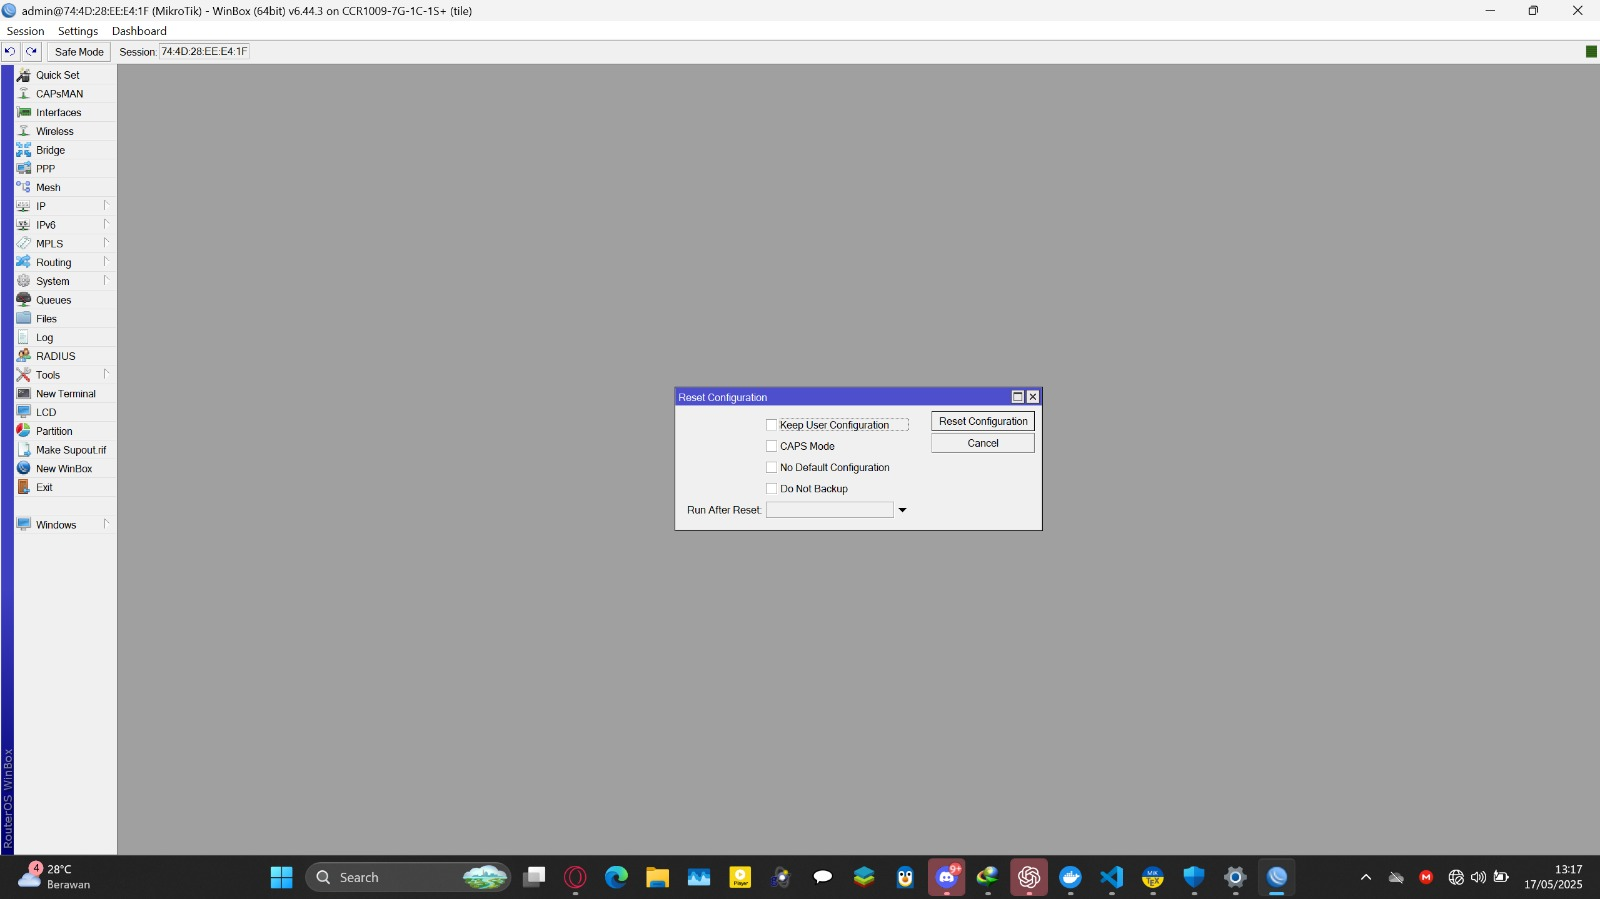
\includegraphics[width=0.5\linewidth]{P1/img/7.jpeg}
    \caption{Reset Configuration}
    \label{fig:inirujukan}
  \end{figure}
  \item Aktifkan IPv6 pada menu
   \begin{figure}[H]
    \centering
    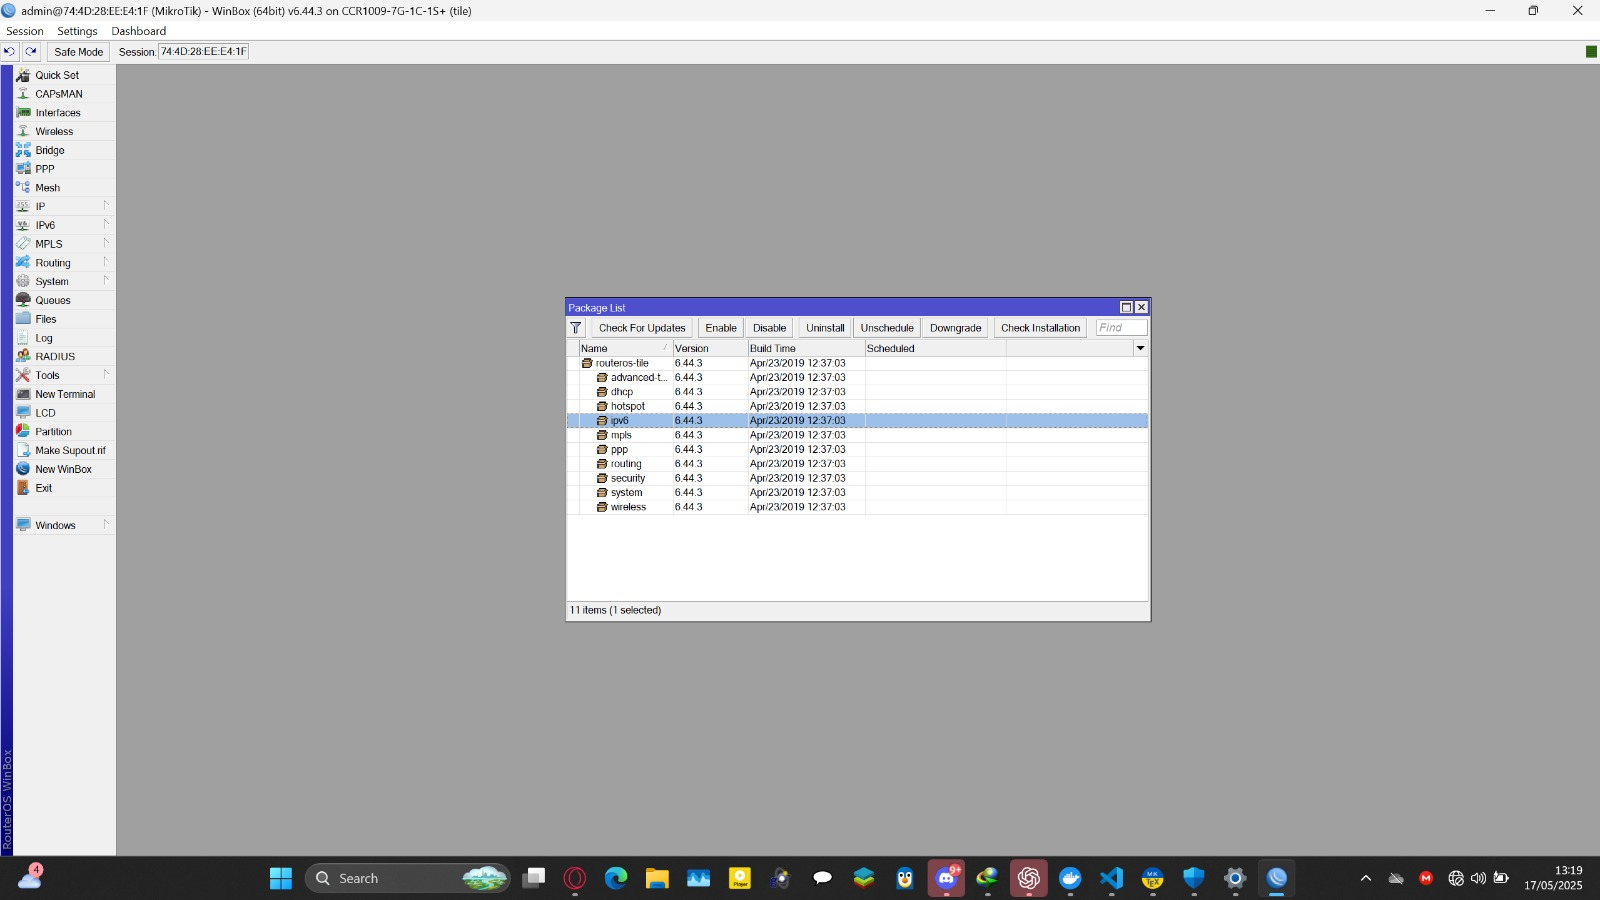
\includegraphics[width=0.5\linewidth]{P1/img/8.jpeg}
    \caption{Pengaktifan IPv6}
    \label{fig:inirujukan}
  \end{figure}
  \item Konfigurasi IP address pada router terhadap ether1 dan ether 2
   \begin{figure}[H]
    \centering
    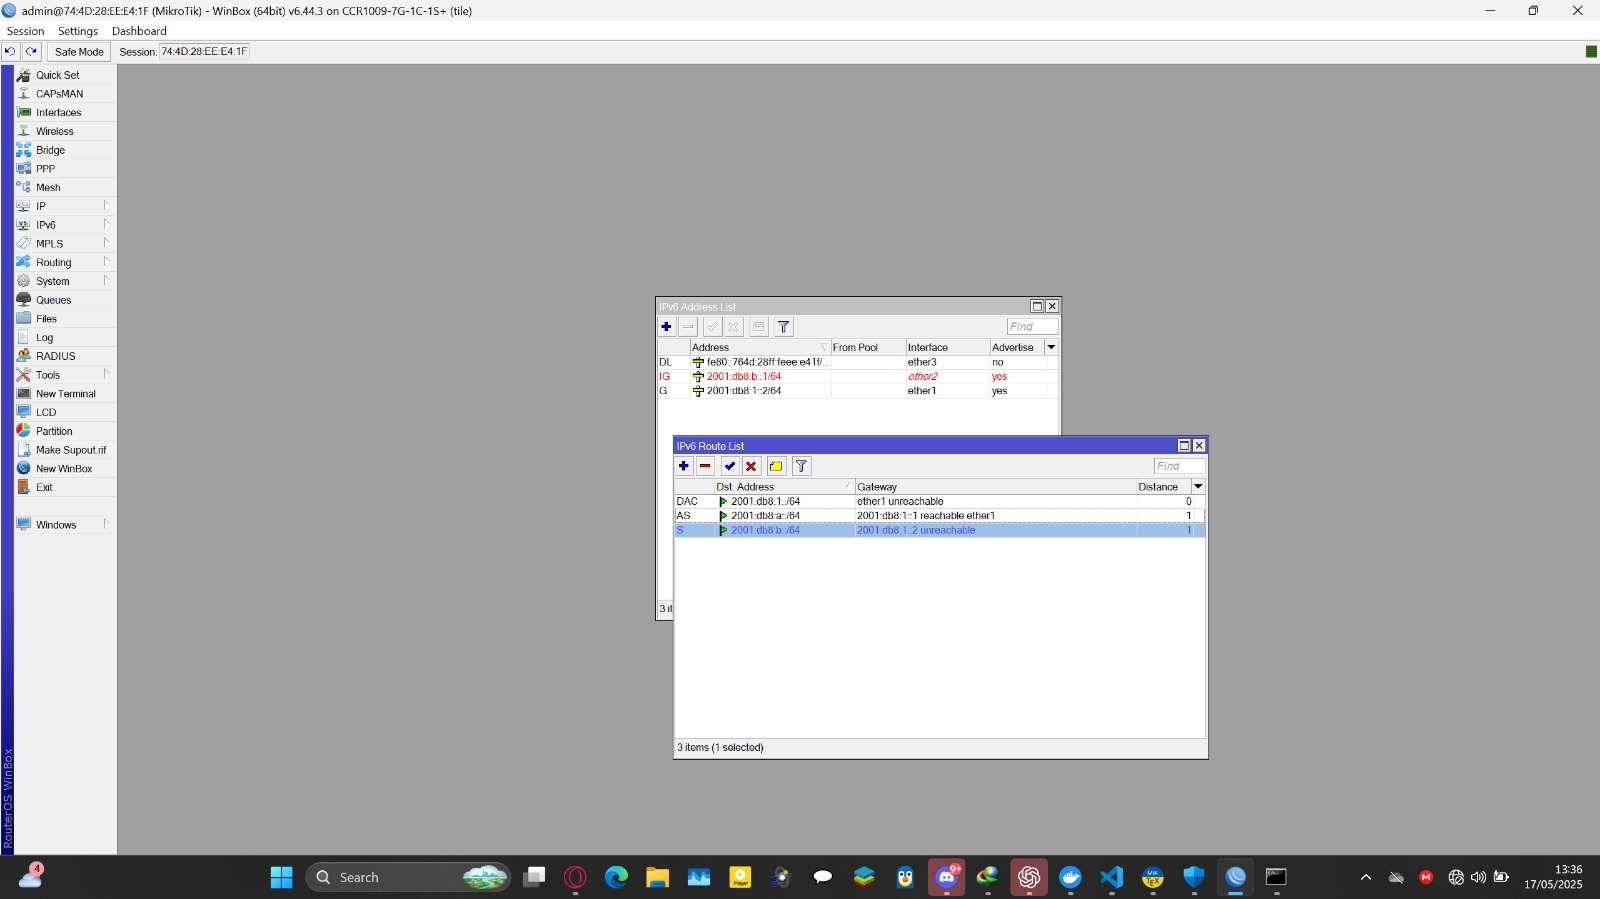
\includegraphics[width=0.5\linewidth]{P1/img/9.jpeg}
    \caption{Hasil konfigurasi}
    \label{fig:inirujukan}
  \end{figure}
  \item Konfigurasi IPv6 pada windows melalui setting ethernet
   \begin{figure}[H]
    \centering
    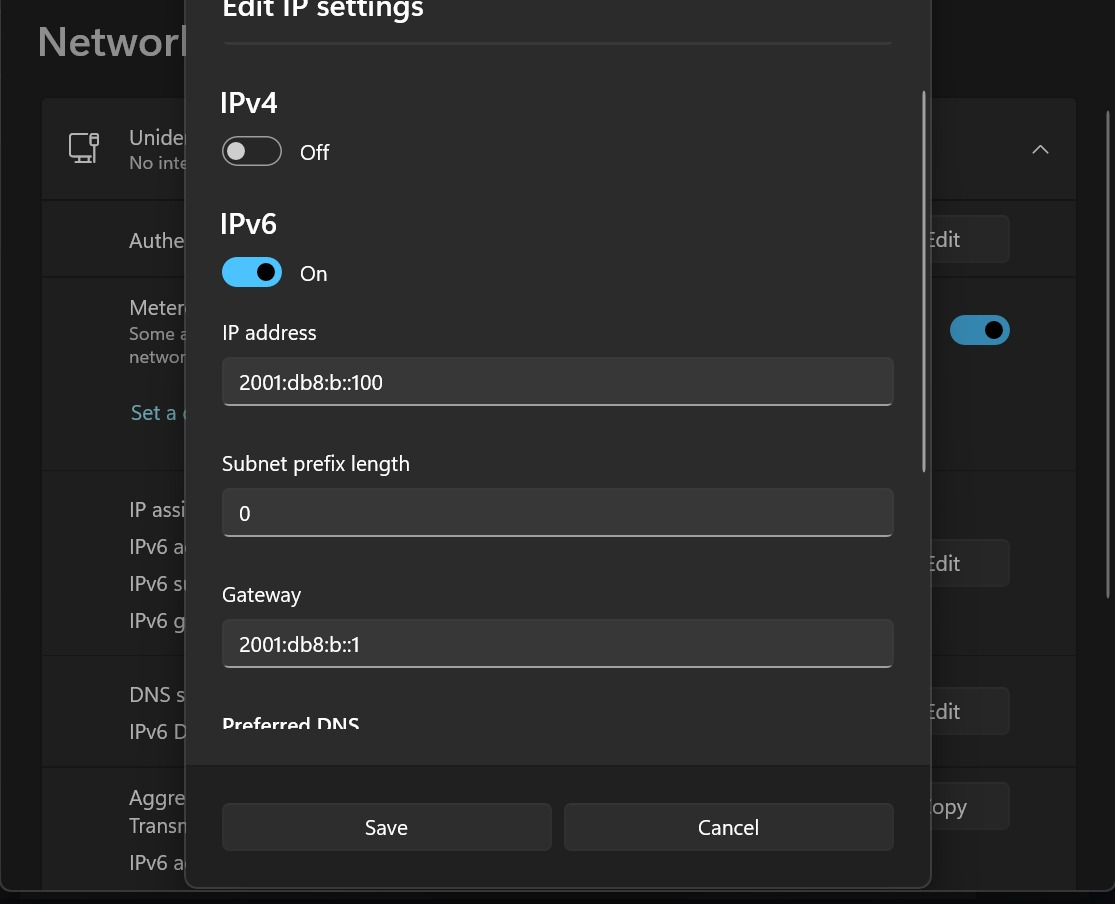
\includegraphics[width=0.5\linewidth]{P1/img/10.jpeg}
    \caption{Konfigurasi pada windows}
    \label{fig:inirujukan}
  \end{figure}
  \item Lakukan uji Ping untuk mengetahui apakah router sudah saling terhubung
   \begin{figure}[H]
    \centering
    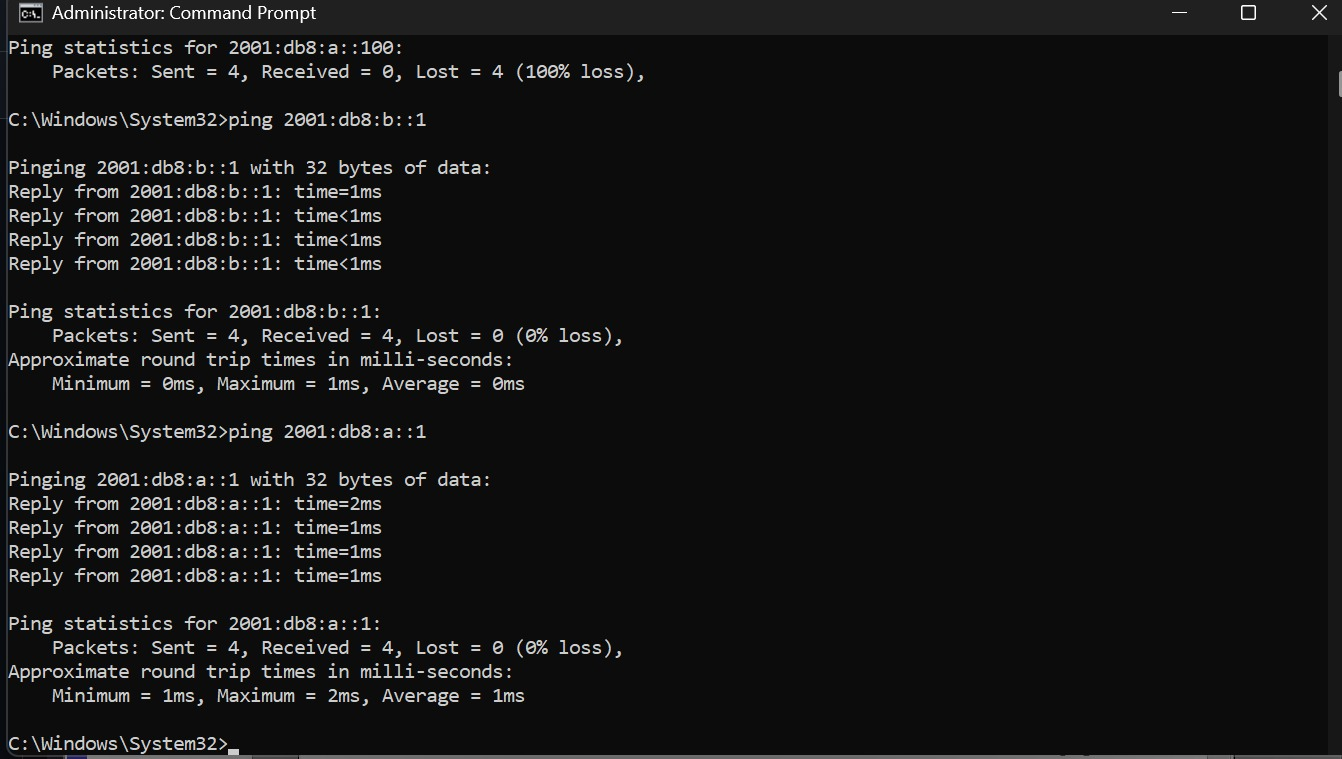
\includegraphics[width=0.5\linewidth]{P1/img/11.jpeg}
    \caption{Laptop dan routher berhasil terhubung}
    \label{fig:inirujukan}
  \end{figure}
\end{enumerate}

\subsection{Routing IPv6 Dinamis}

\begin{enumerate}
  
  \item Sebelum memulai praktikum, lakukan reset configuration melalui winbox
   \begin{figure}[H]
    \centering
    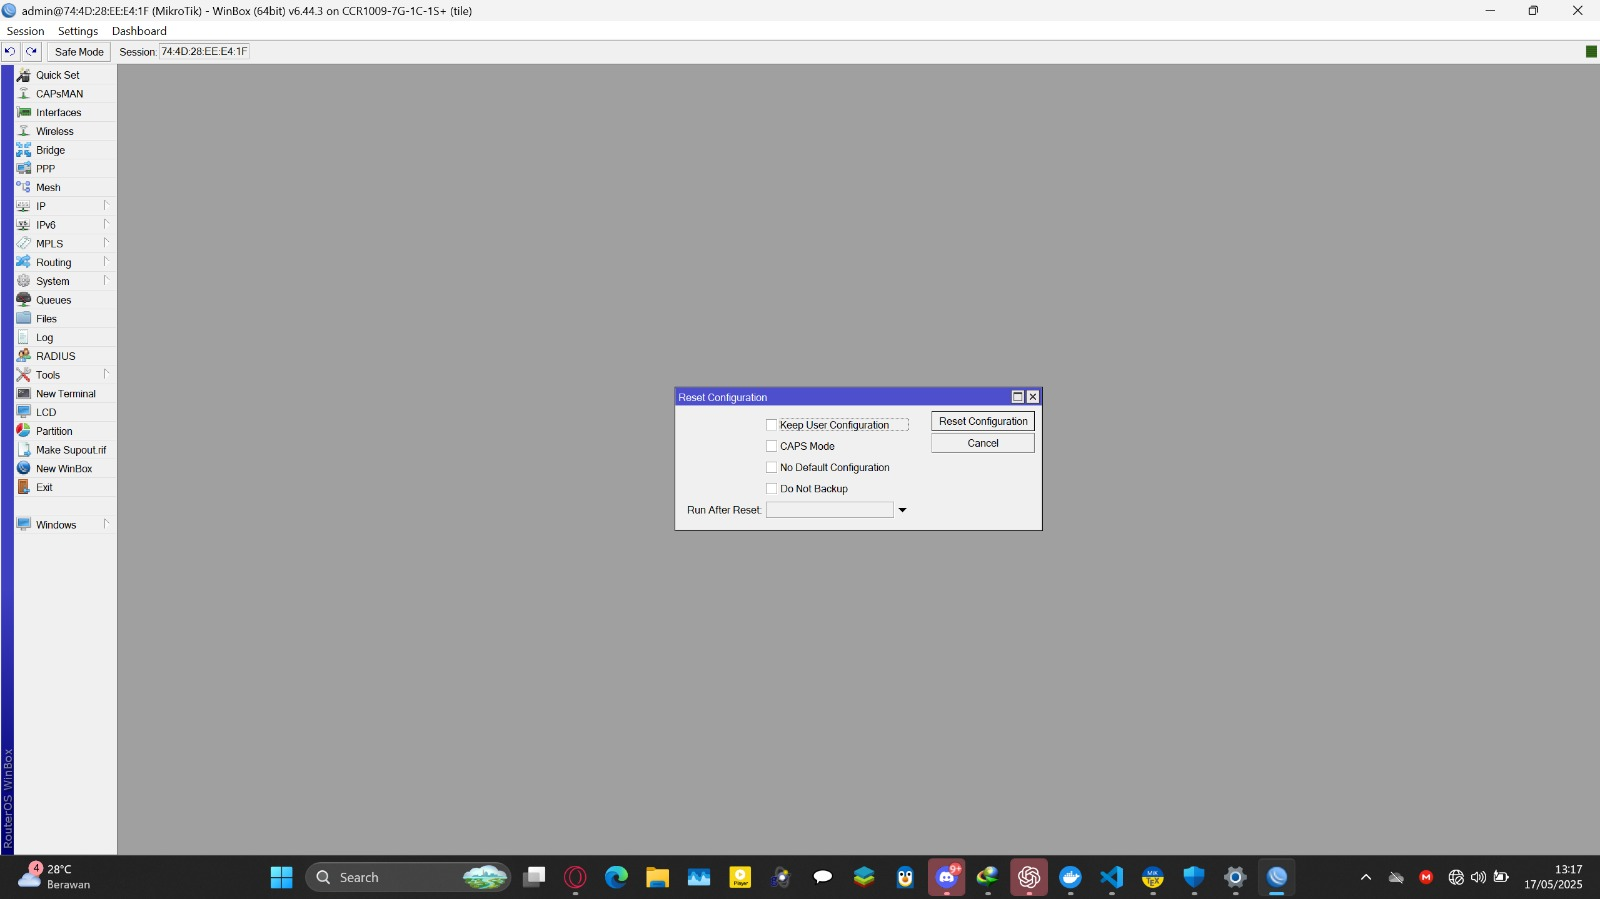
\includegraphics[width=0.5\linewidth]{P1/img/7.jpeg}
    \caption{Reset Configuration}
    \label{fig:inirujukan}
  \end{figure}
  \item Aktifkan IPv6 pada menu
   \begin{figure}[H]
    \centering
    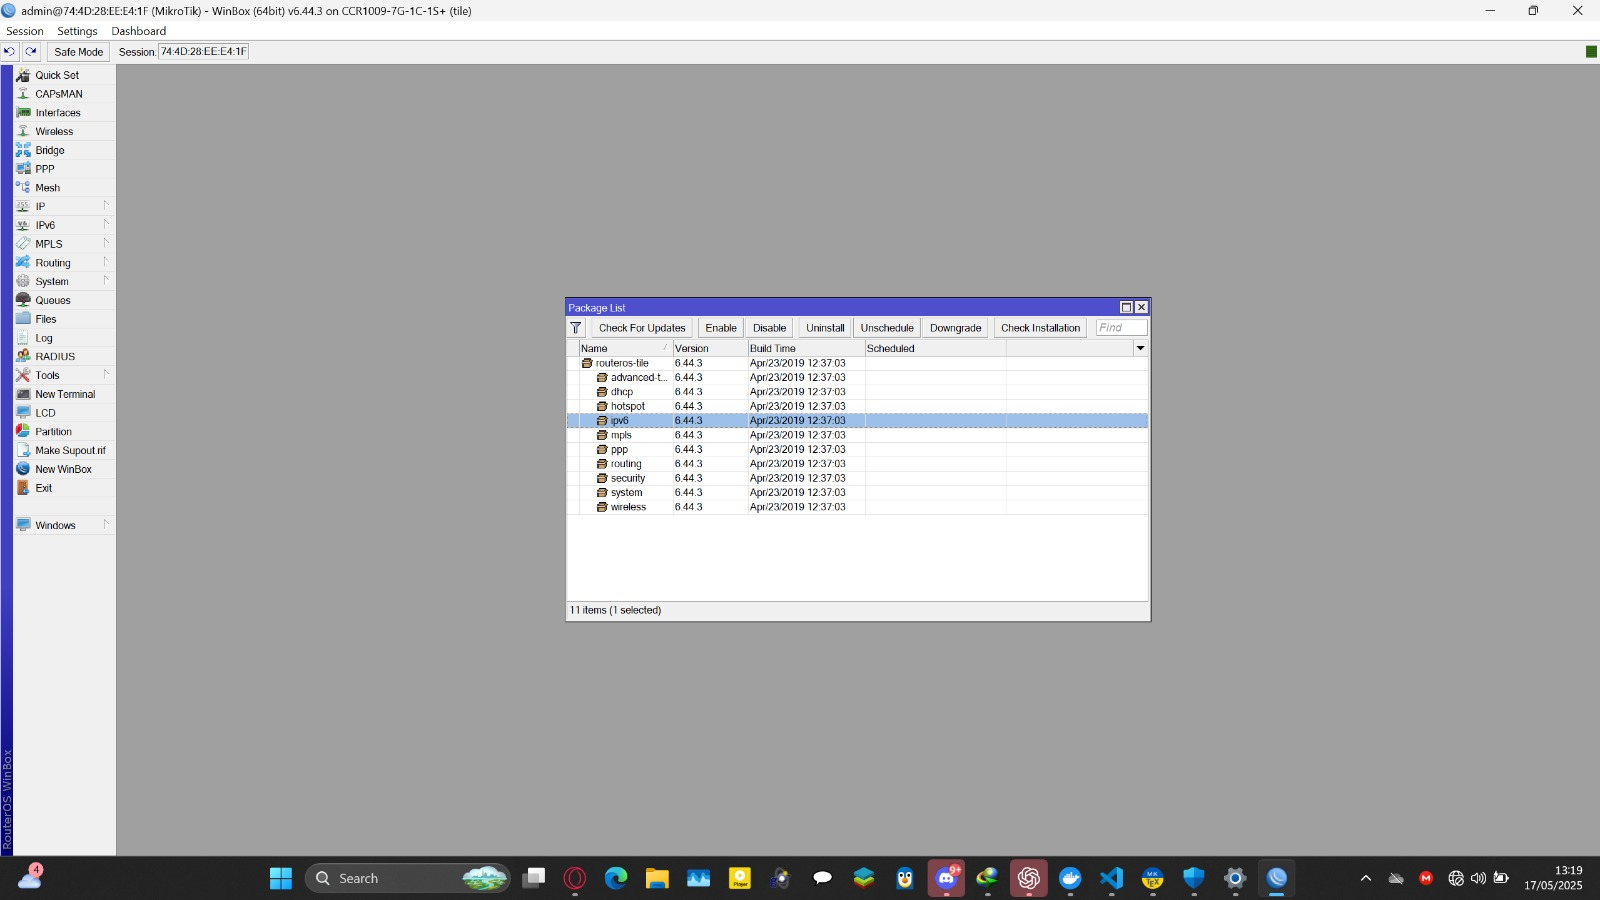
\includegraphics[width=0.5\linewidth]{P1/img/8.jpeg}
    \caption{Pengaktifan IPv6}
    \label{fig:inirujukan}
  \end{figure}
  \item Konfigurasi IP address pada router terhadap ether1 dan ether 2
   \begin{figure}[H]
    \centering
    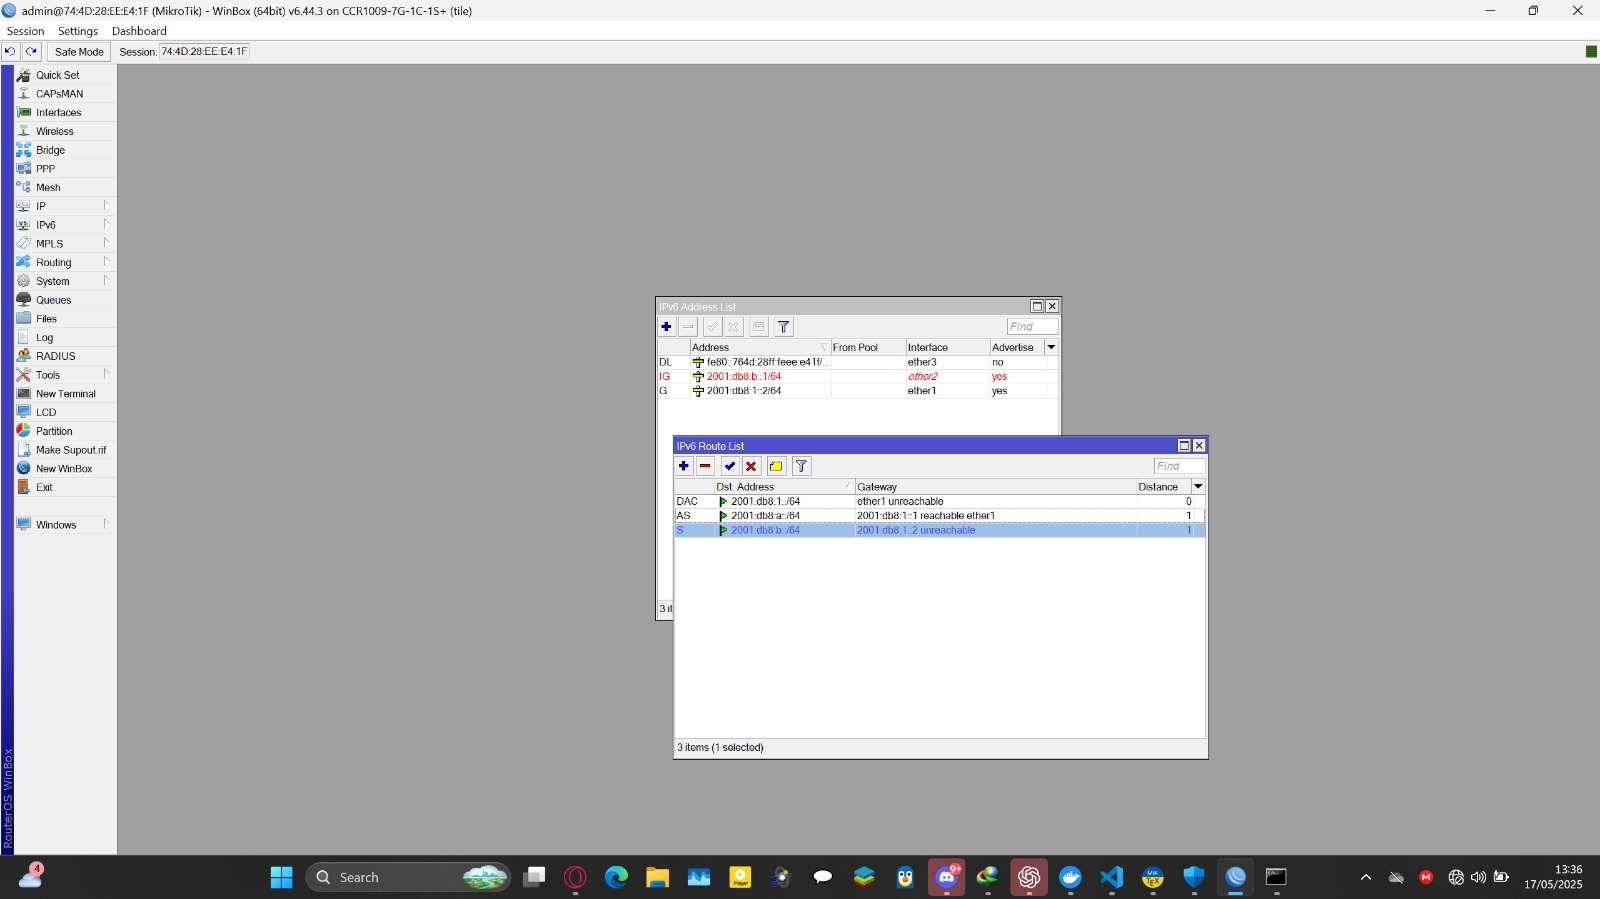
\includegraphics[width=0.5\linewidth]{P1/img/9.jpeg}
    \caption{Hasil konfigurasi}
    \label{fig:inirujukan}
  \end{figure}
\item Buatlah sebuah instance OSPF melalui menu OSPF Instance dan beri nama ospf-instance.
    \begin{figure}[H]
        \centering
        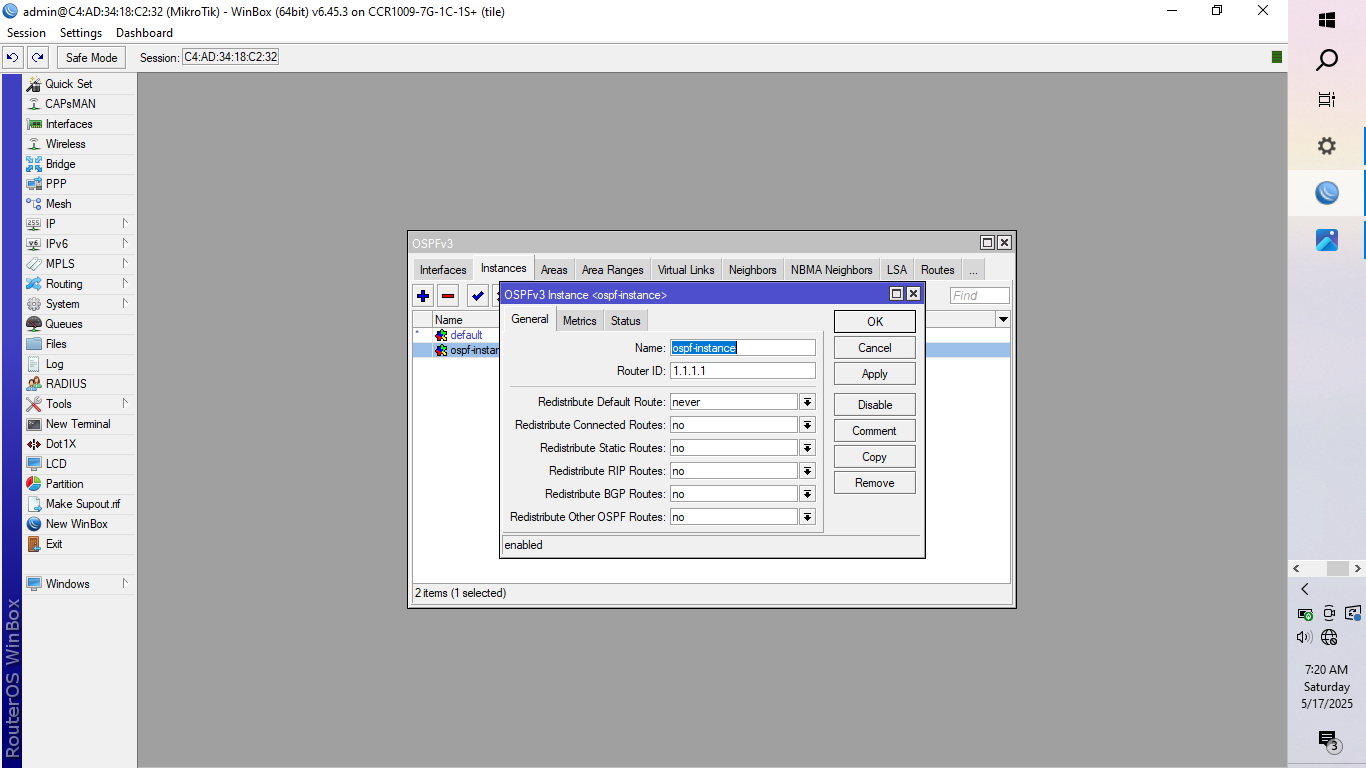
\includegraphics[width=0.5\linewidth]{P1/gambar5.png}
        \caption{Membuat Instance OSPF pada Router}
        \label{fig:gambar6}
    \end{figure}    
    \item Selanjutnya, tambahkan area OSPF melalui menu OSPF Area dengan nama area1.
    \begin{figure}[H]
        \centering
        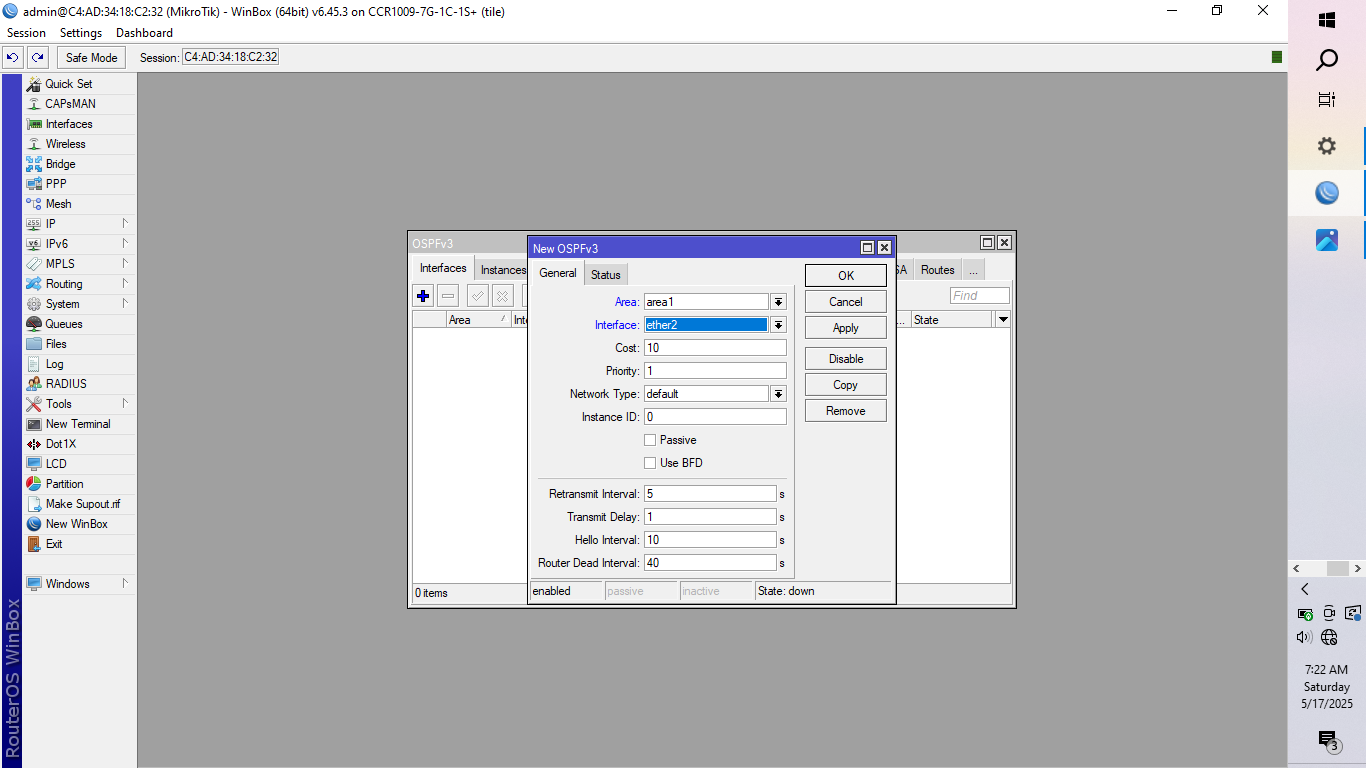
\includegraphics[width=0.5\linewidth]{P1/gambar6.png}
        \caption{Menambahkan Area OSPF pada Router}
        \label{fig:gambar7}
    \end{figure}
    \item Masukkan setiap interface router ke dalam OSPF melalui menu OSPF Interface. router.
    \begin{figure}[H]
        \centering
        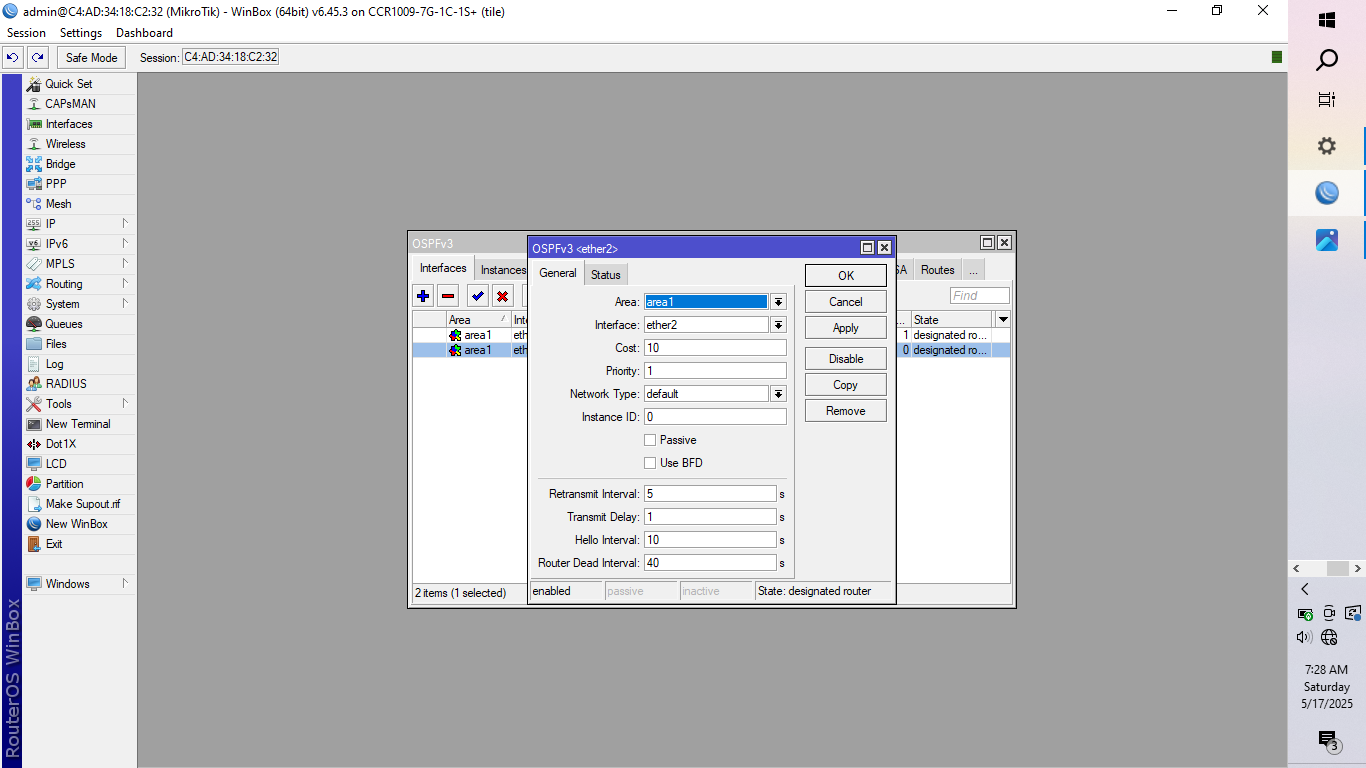
\includegraphics[width=0.5\linewidth]{P1/gambar7.png}
        \caption{Menambahkan Interface OSPF pada Router}
        \label{fig:gambar8}
    \end{figure}
        \item Atur konfigurasi IPv6 pada laptop sesuai alamat IPv6 yang telah ditentukan melalui menu Settings pada perangkat laptop.
    \begin{figure}[H]
        \centering
        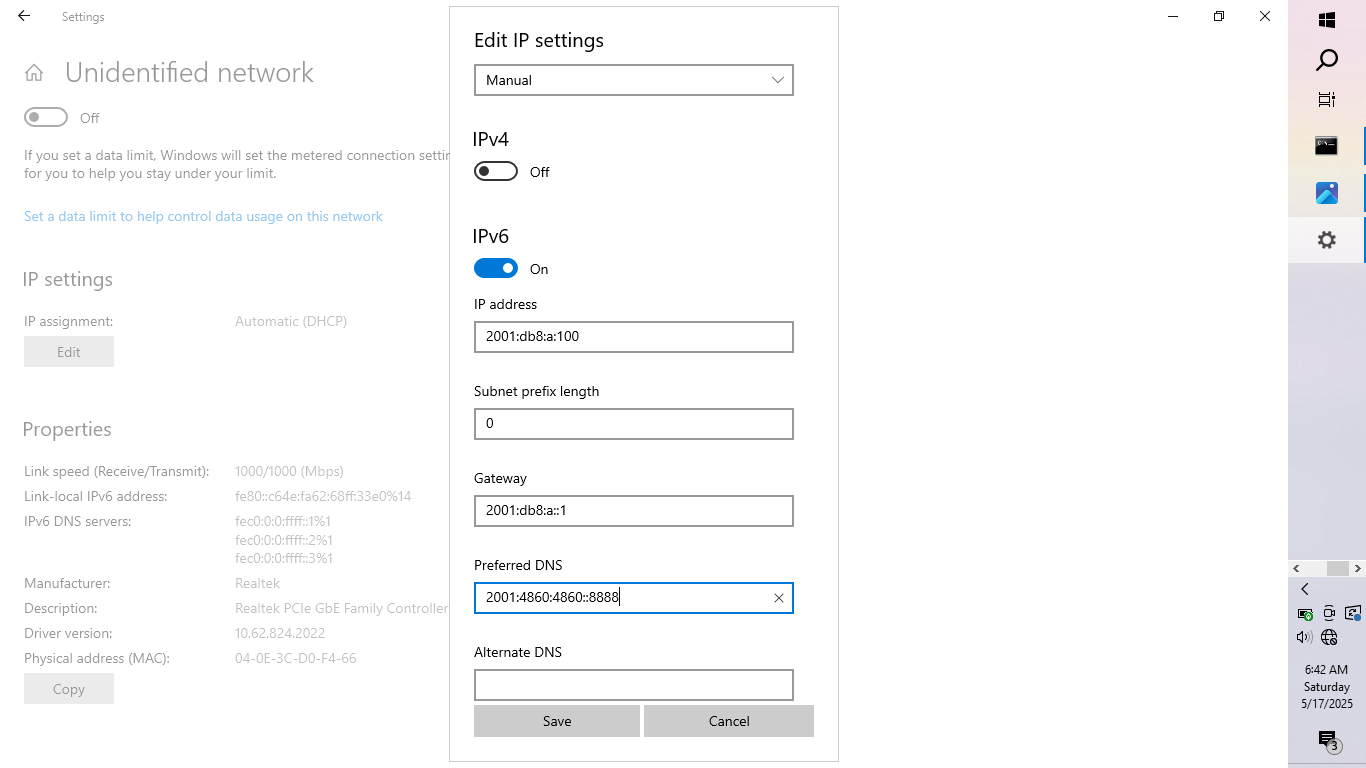
\includegraphics[width=0.5\linewidth]{P1/gambar4.png}
        \caption{Mengkonfigurasi IPv6 pada Laptop}
        \label{fig:gambar4}
    \end{figure}
    \item Setelah seluruh konfigurasi selesai, lakukan pengujian koneksi dengan perintah ping dari laptop ke router dan ke laptop lainnya untuk memastikan jaringan antar perangkat telah terhubung dengan baik.
    \begin{figure}[H]
        \centering
        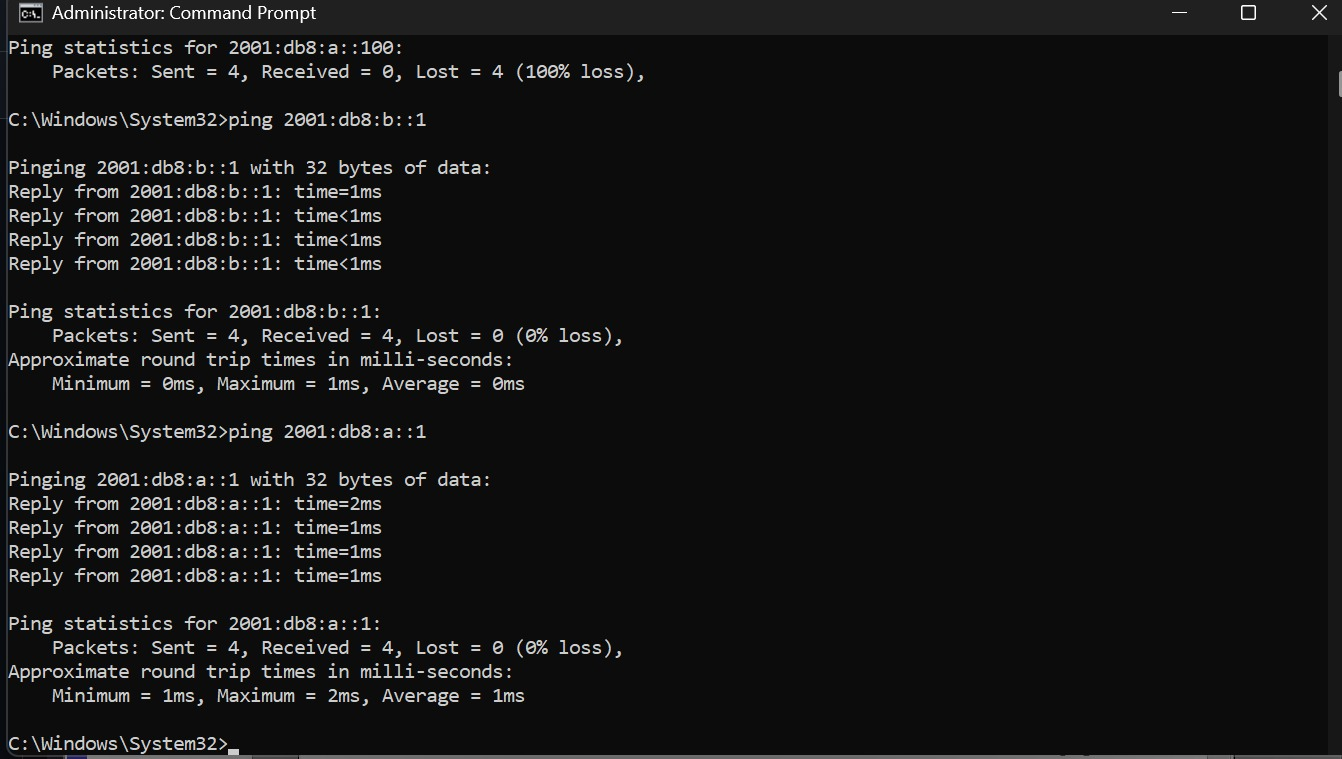
\includegraphics[width=0.5\linewidth]{P1/img/11.jpeg}
        \caption{Melakukan Ping dari Laptop ke Router}
        \label{fig:gambar5}
    \end{figure}

  
\end{enumerate}



\section{Analisis Hasil Percobaan}
Pada praktikum konfigurasi routing IPv6, baik metode statis maupun dinamis berhasil diimplementasikan dengan baik. Hal ini dibuktikan melalui hasil pengujian konektivitas antarlaptop dan antarrouter yang menunjukkan respons sukses terhadap perintah \texttt{ping}. Ketika routing statis diterapkan, setiap rute harus dikonfigurasi secara manual pada masing-masing router, termasuk penentuan alamat tujuan dan gateway yang sesuai. Meskipun berhasil menghubungkan antarjaringan, pendekatan ini memerlukan ketelitian tinggi dan rawan kesalahan jika terjadi perubahan pada topologi jaringan.

Sebaliknya, pada penerapan routing dinamis menggunakan OSPFv3, proses konfigurasi menjadi lebih fleksibel dan adaptif. Setelah instance OSPF dan area backbone dibuat, serta interface yang relevan dimasukkan ke dalam konfigurasi OSPF, masing-masing router mampu mendeteksi tetangga secara otomatis dan membentuk tabel rute tanpa perlu input manual. Ini terbukti ketika rute-rute baru muncul dalam daftar routing IPv6 dan proses \texttt{ping} antarhost tetap sukses dilakukan. Pendekatan ini tidak hanya mengurangi beban administrasi, tetapi juga lebih tangguh terhadap perubahan jaringan karena setiap router dapat memperbarui informasi topologi secara real-time.

Secara keseluruhan, hasil praktikum menunjukkan bahwa kedua metode routing dapat digunakan untuk mencapai konektivitas antarlaptop yang terhubung melalui dua router, namun dari sisi efisiensi dan skalabilitas, routing dinamis menawarkan keunggulan yang lebih signifikan. Dalam lingkungan jaringan yang kompleks dan sering mengalami perubahan, protokol seperti OSPFv3 menjadi solusi yang lebih layak dibandingkan dengan pendekatan statis yang kurang fleksibel.

\section{Hasil Tugas Modul}
\begin{enumerate}
    \item Simulasikan Konfigurasi Praktikum P2 di atas mengenai Routing Dinamis dan Statis IPV6 menggunakan GNS3
    \\ Dinamis:
    \begin{figure}[H]
        \centering
        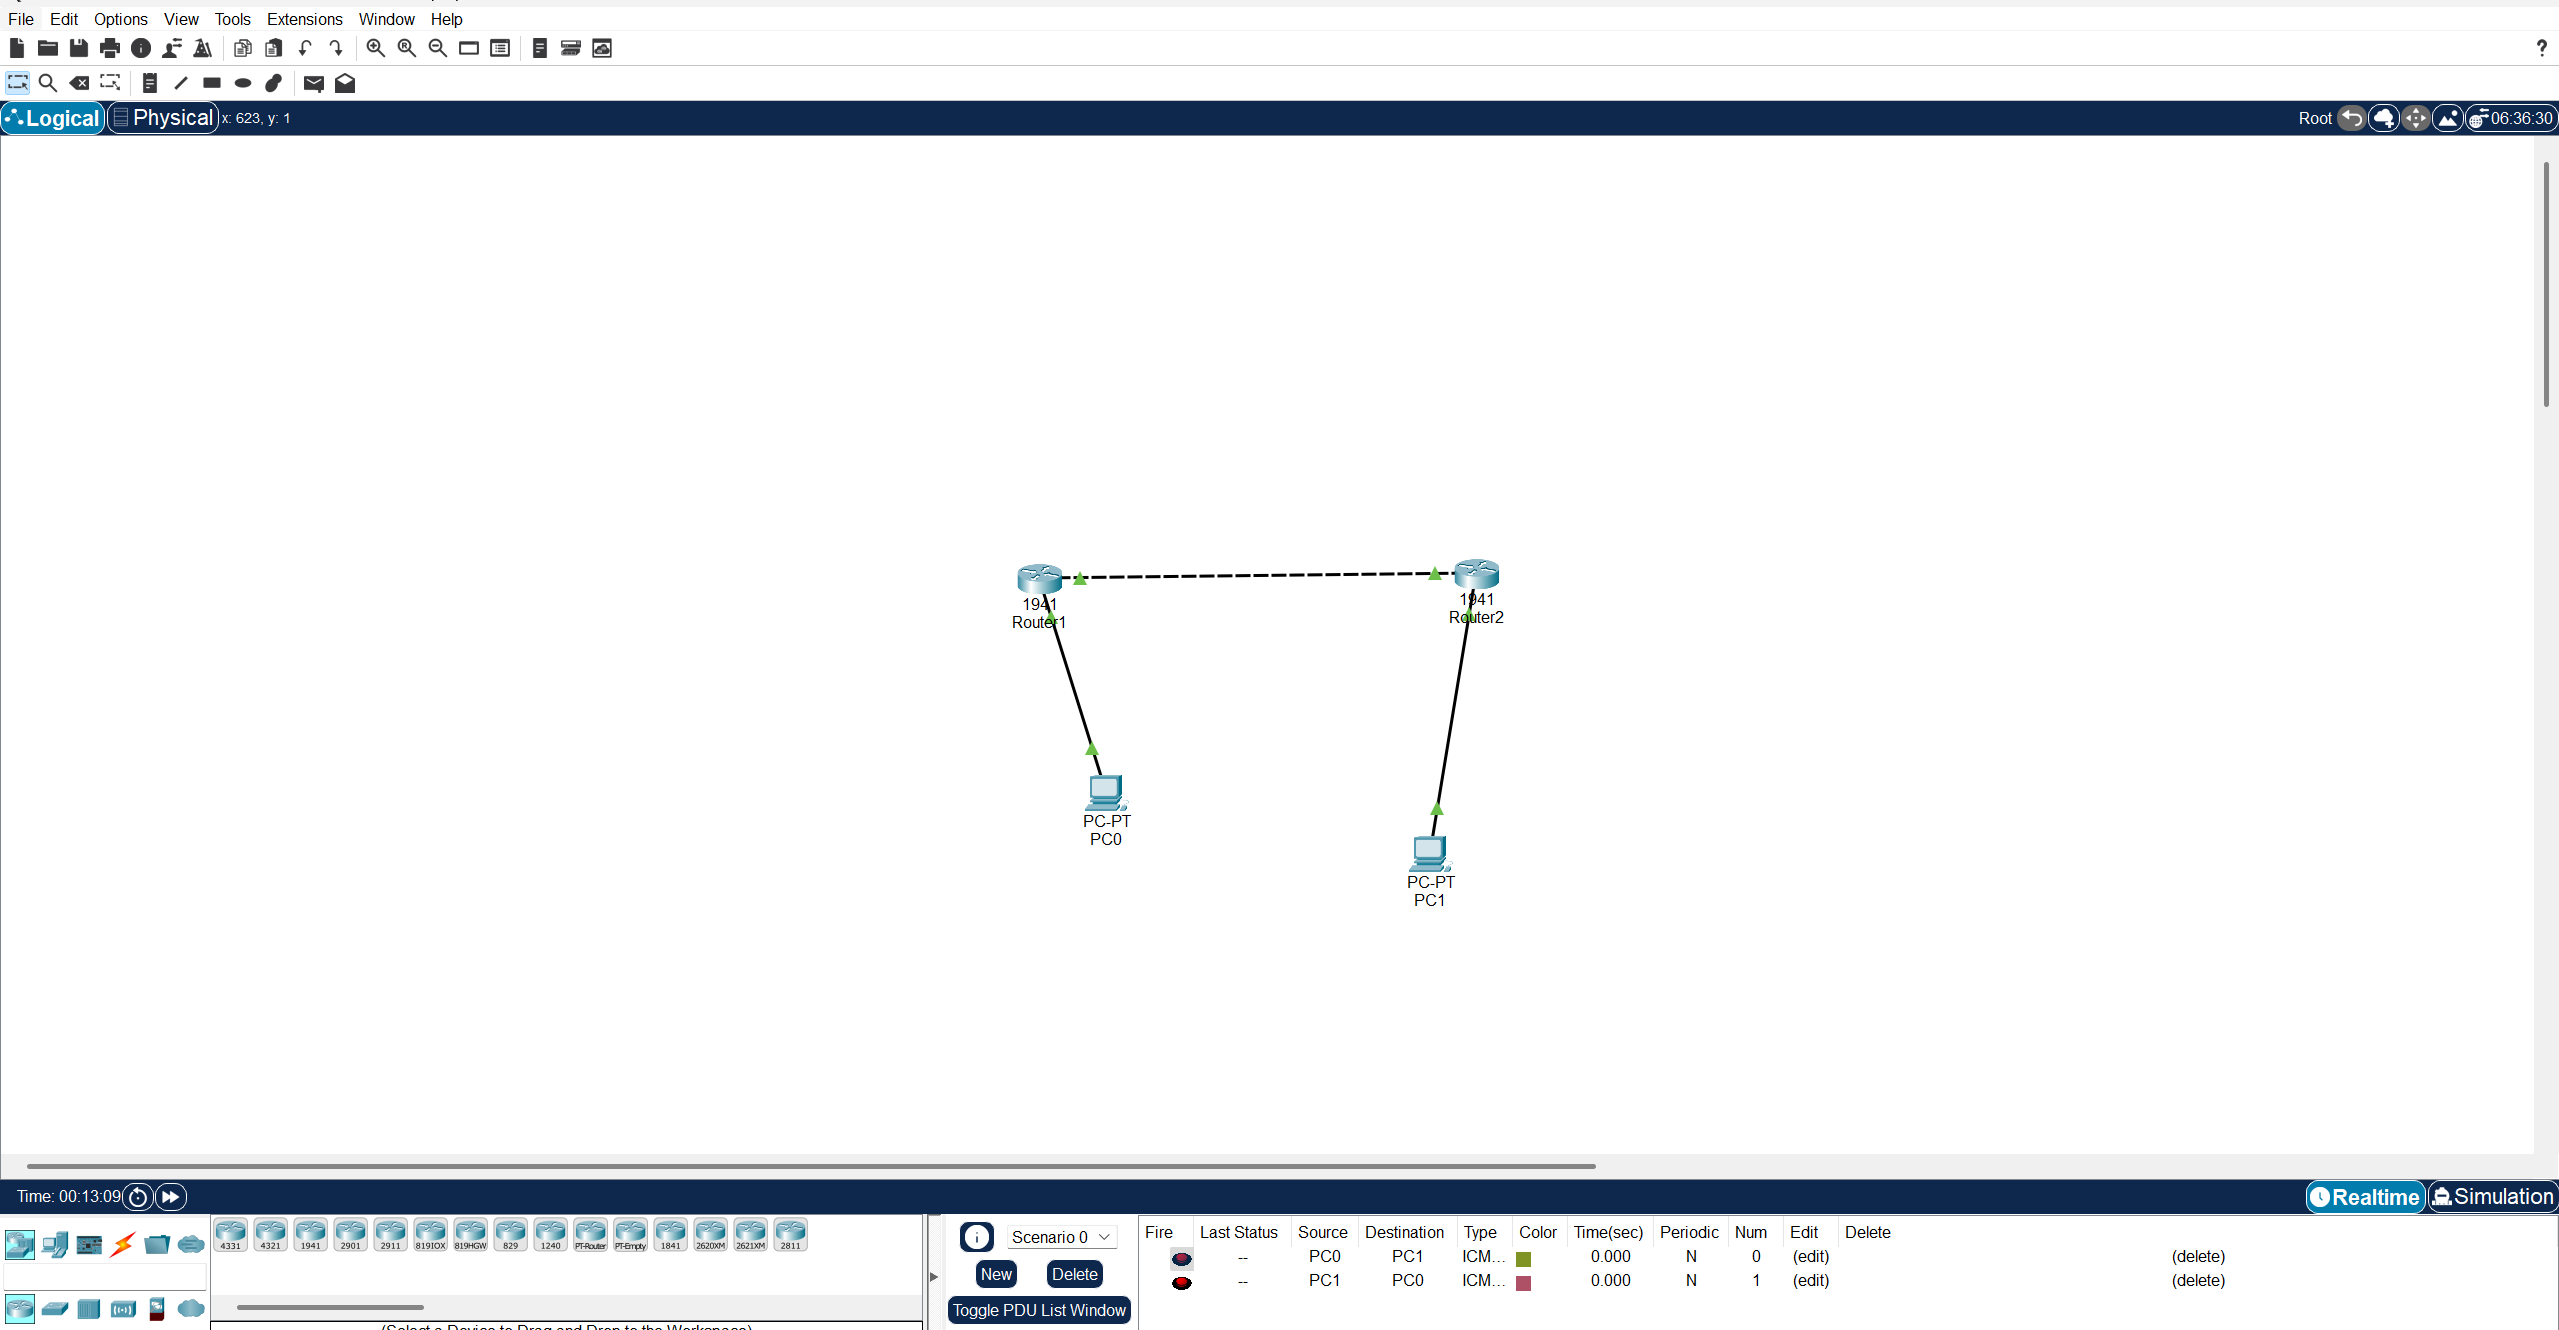
\includegraphics[width=0.5\linewidth]{P1/img/12.png}
        \caption{Dinamis}
        \label{fig:gambar4}
    \end{figure}
  \\ Statis:
  \begin{figure}[H]
        \centering
        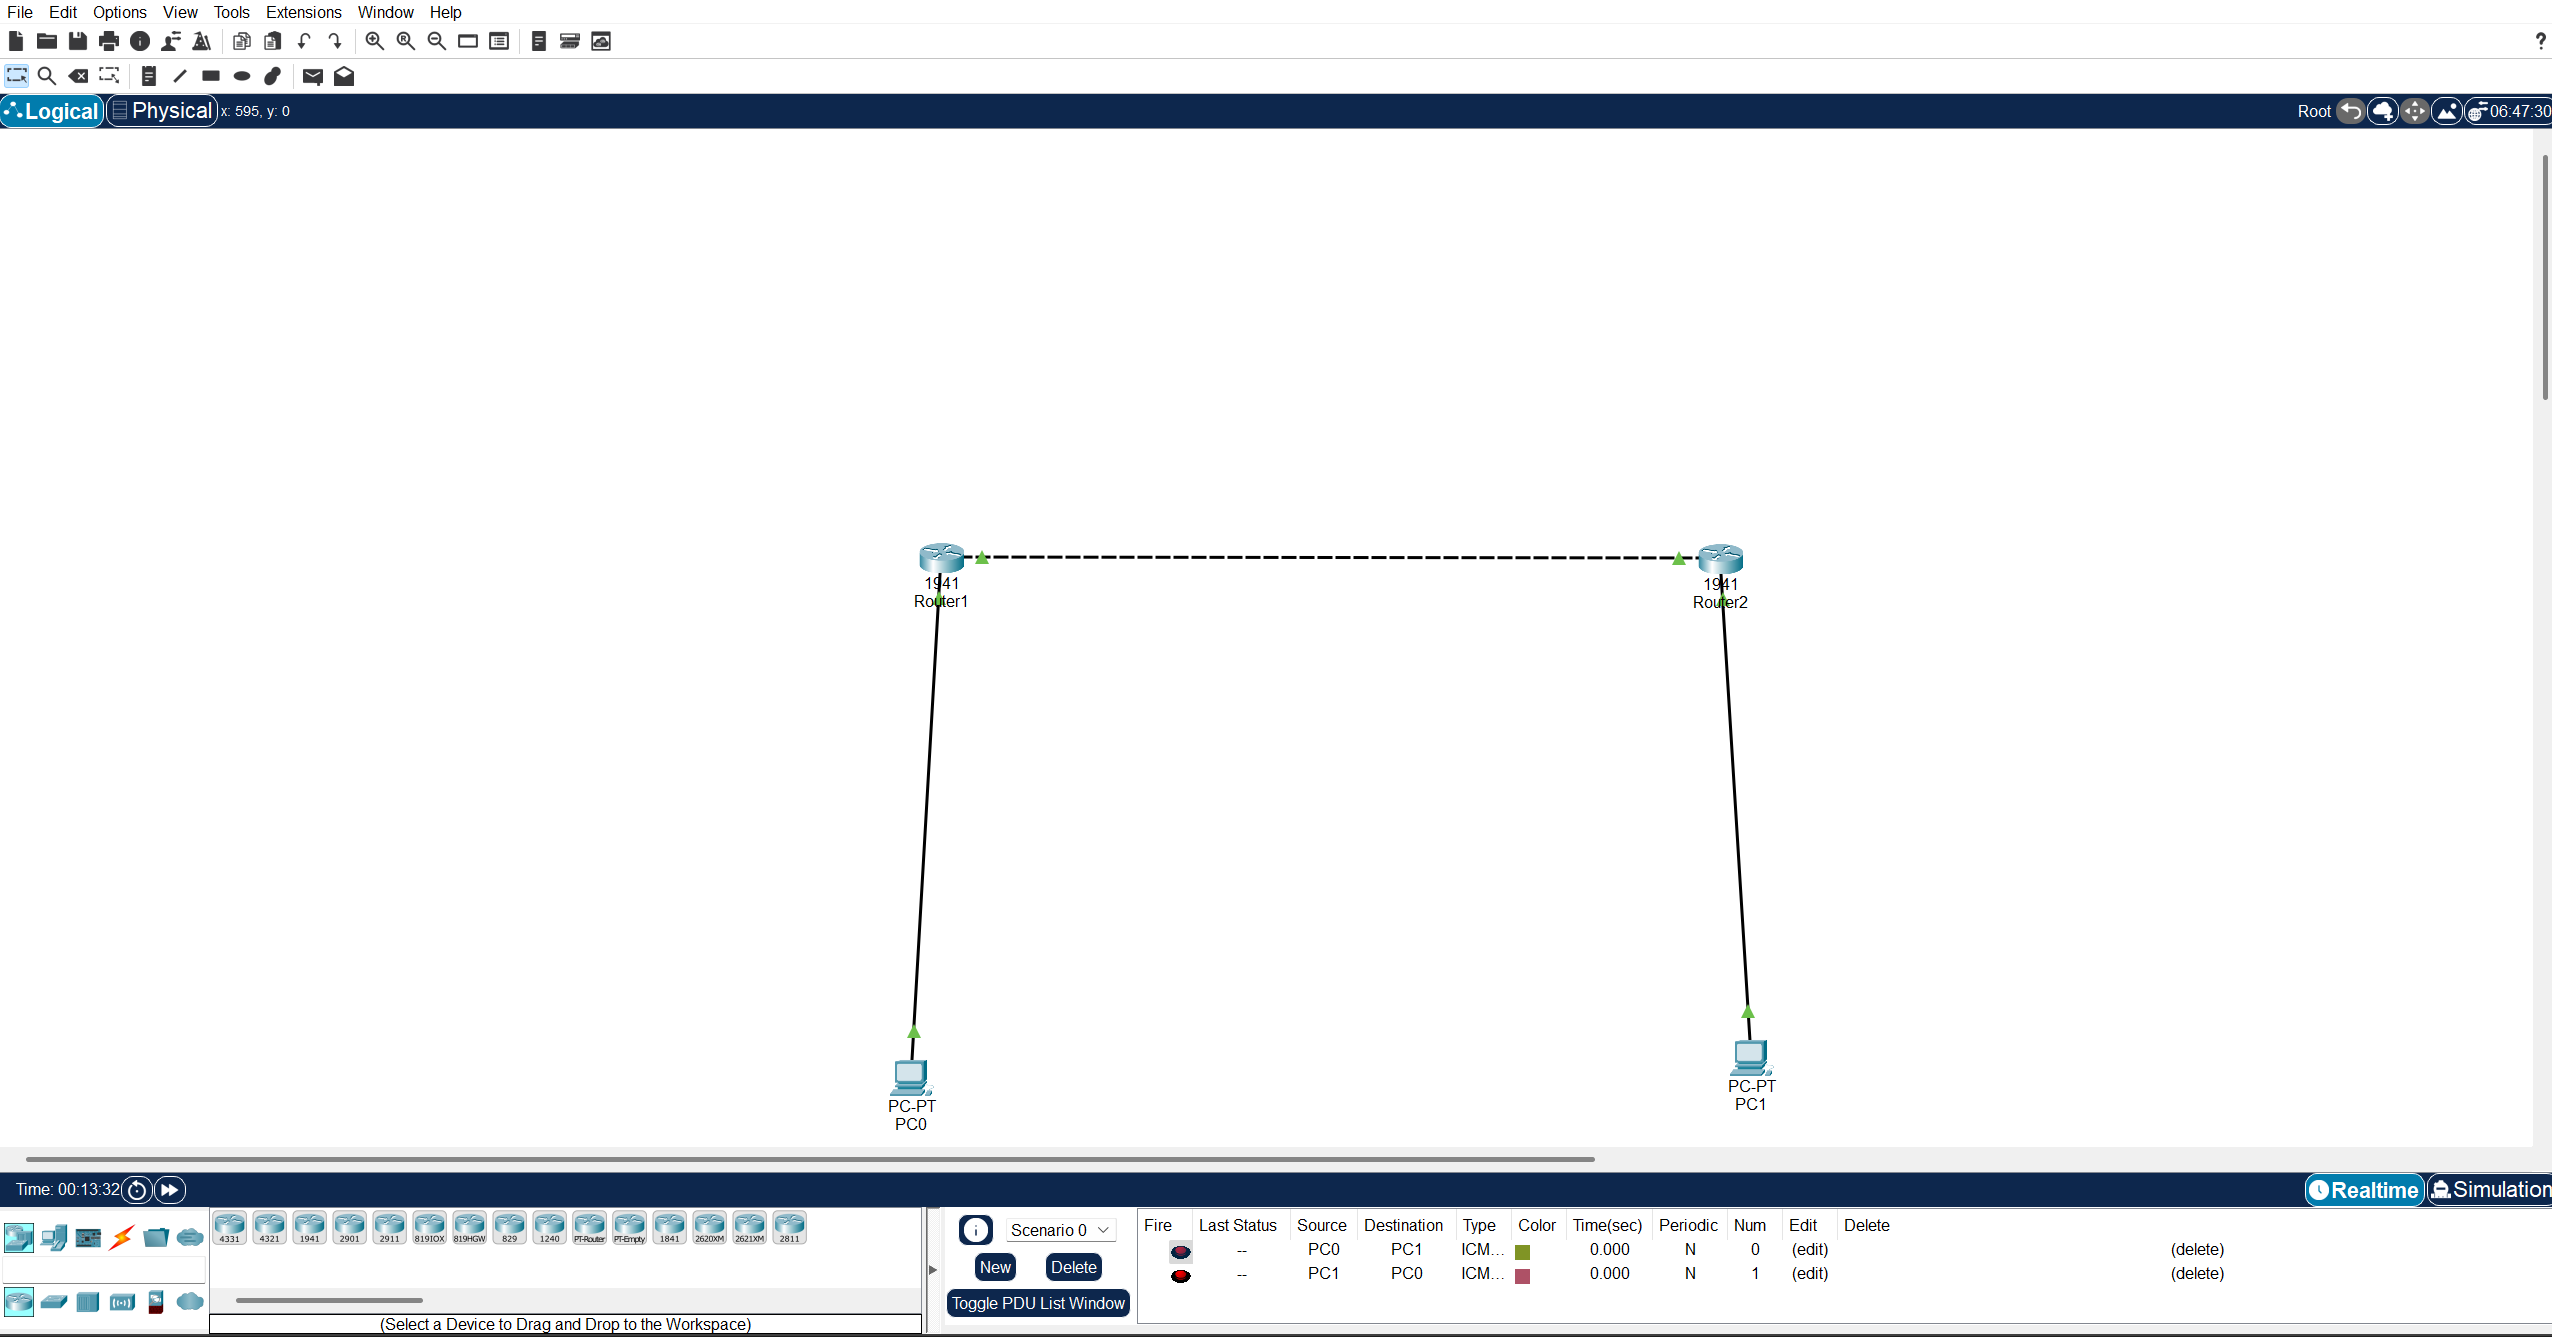
\includegraphics[width=0.5\linewidth]{P1/img/13.png}
        \caption{Statis}
        \label{fig:gambar4}
    \end{figure}
  
  

\end{enumerate}

\section{Kesimpulan}
Dari praktikum yang telah dilakukan, dapat disimpulkan bahwa pemahaman dan implementasi routing IPv6, baik secara statis maupun dinamis, sangat penting dalam membangun konektivitas jaringan yang stabil dan efisien. Pada skenario routing statis, konfigurasi manual memberikan kendali penuh terhadap arah lalu lintas jaringan, namun menuntut ketelitian ekstra karena kesalahan kecil dapat menyebabkan kegagalan koneksi antarperangkat. Praktikum menunjukkan bahwa setiap entri rute harus ditentukan secara eksplisit agar perangkat dapat saling berkomunikasi.

Sementara itu, pada implementasi routing dinamis menggunakan OSPFv3, proses distribusi informasi jaringan menjadi lebih otomatis dan responsif terhadap perubahan topologi. Router secara mandiri dapat membangun tabel routing dan mendeteksi perubahan jaringan tanpa perlu konfigurasi manual yang berulang. Hal ini menjadikan routing dinamis lebih praktis diterapkan, terutama pada jaringan berskala besar atau yang dinamis. Secara keseluruhan, praktikum ini memberikan wawasan praktis mengenai kelebihan dan kekurangan masing-masing metode routing, serta pentingnya perencanaan dan pengujian dalam membangun jaringan IPv6 yang andal.


\section{Lampiran}
\subsection{Dokumentasi saat praktikum}
\begin{figure}[H]
        \centering
        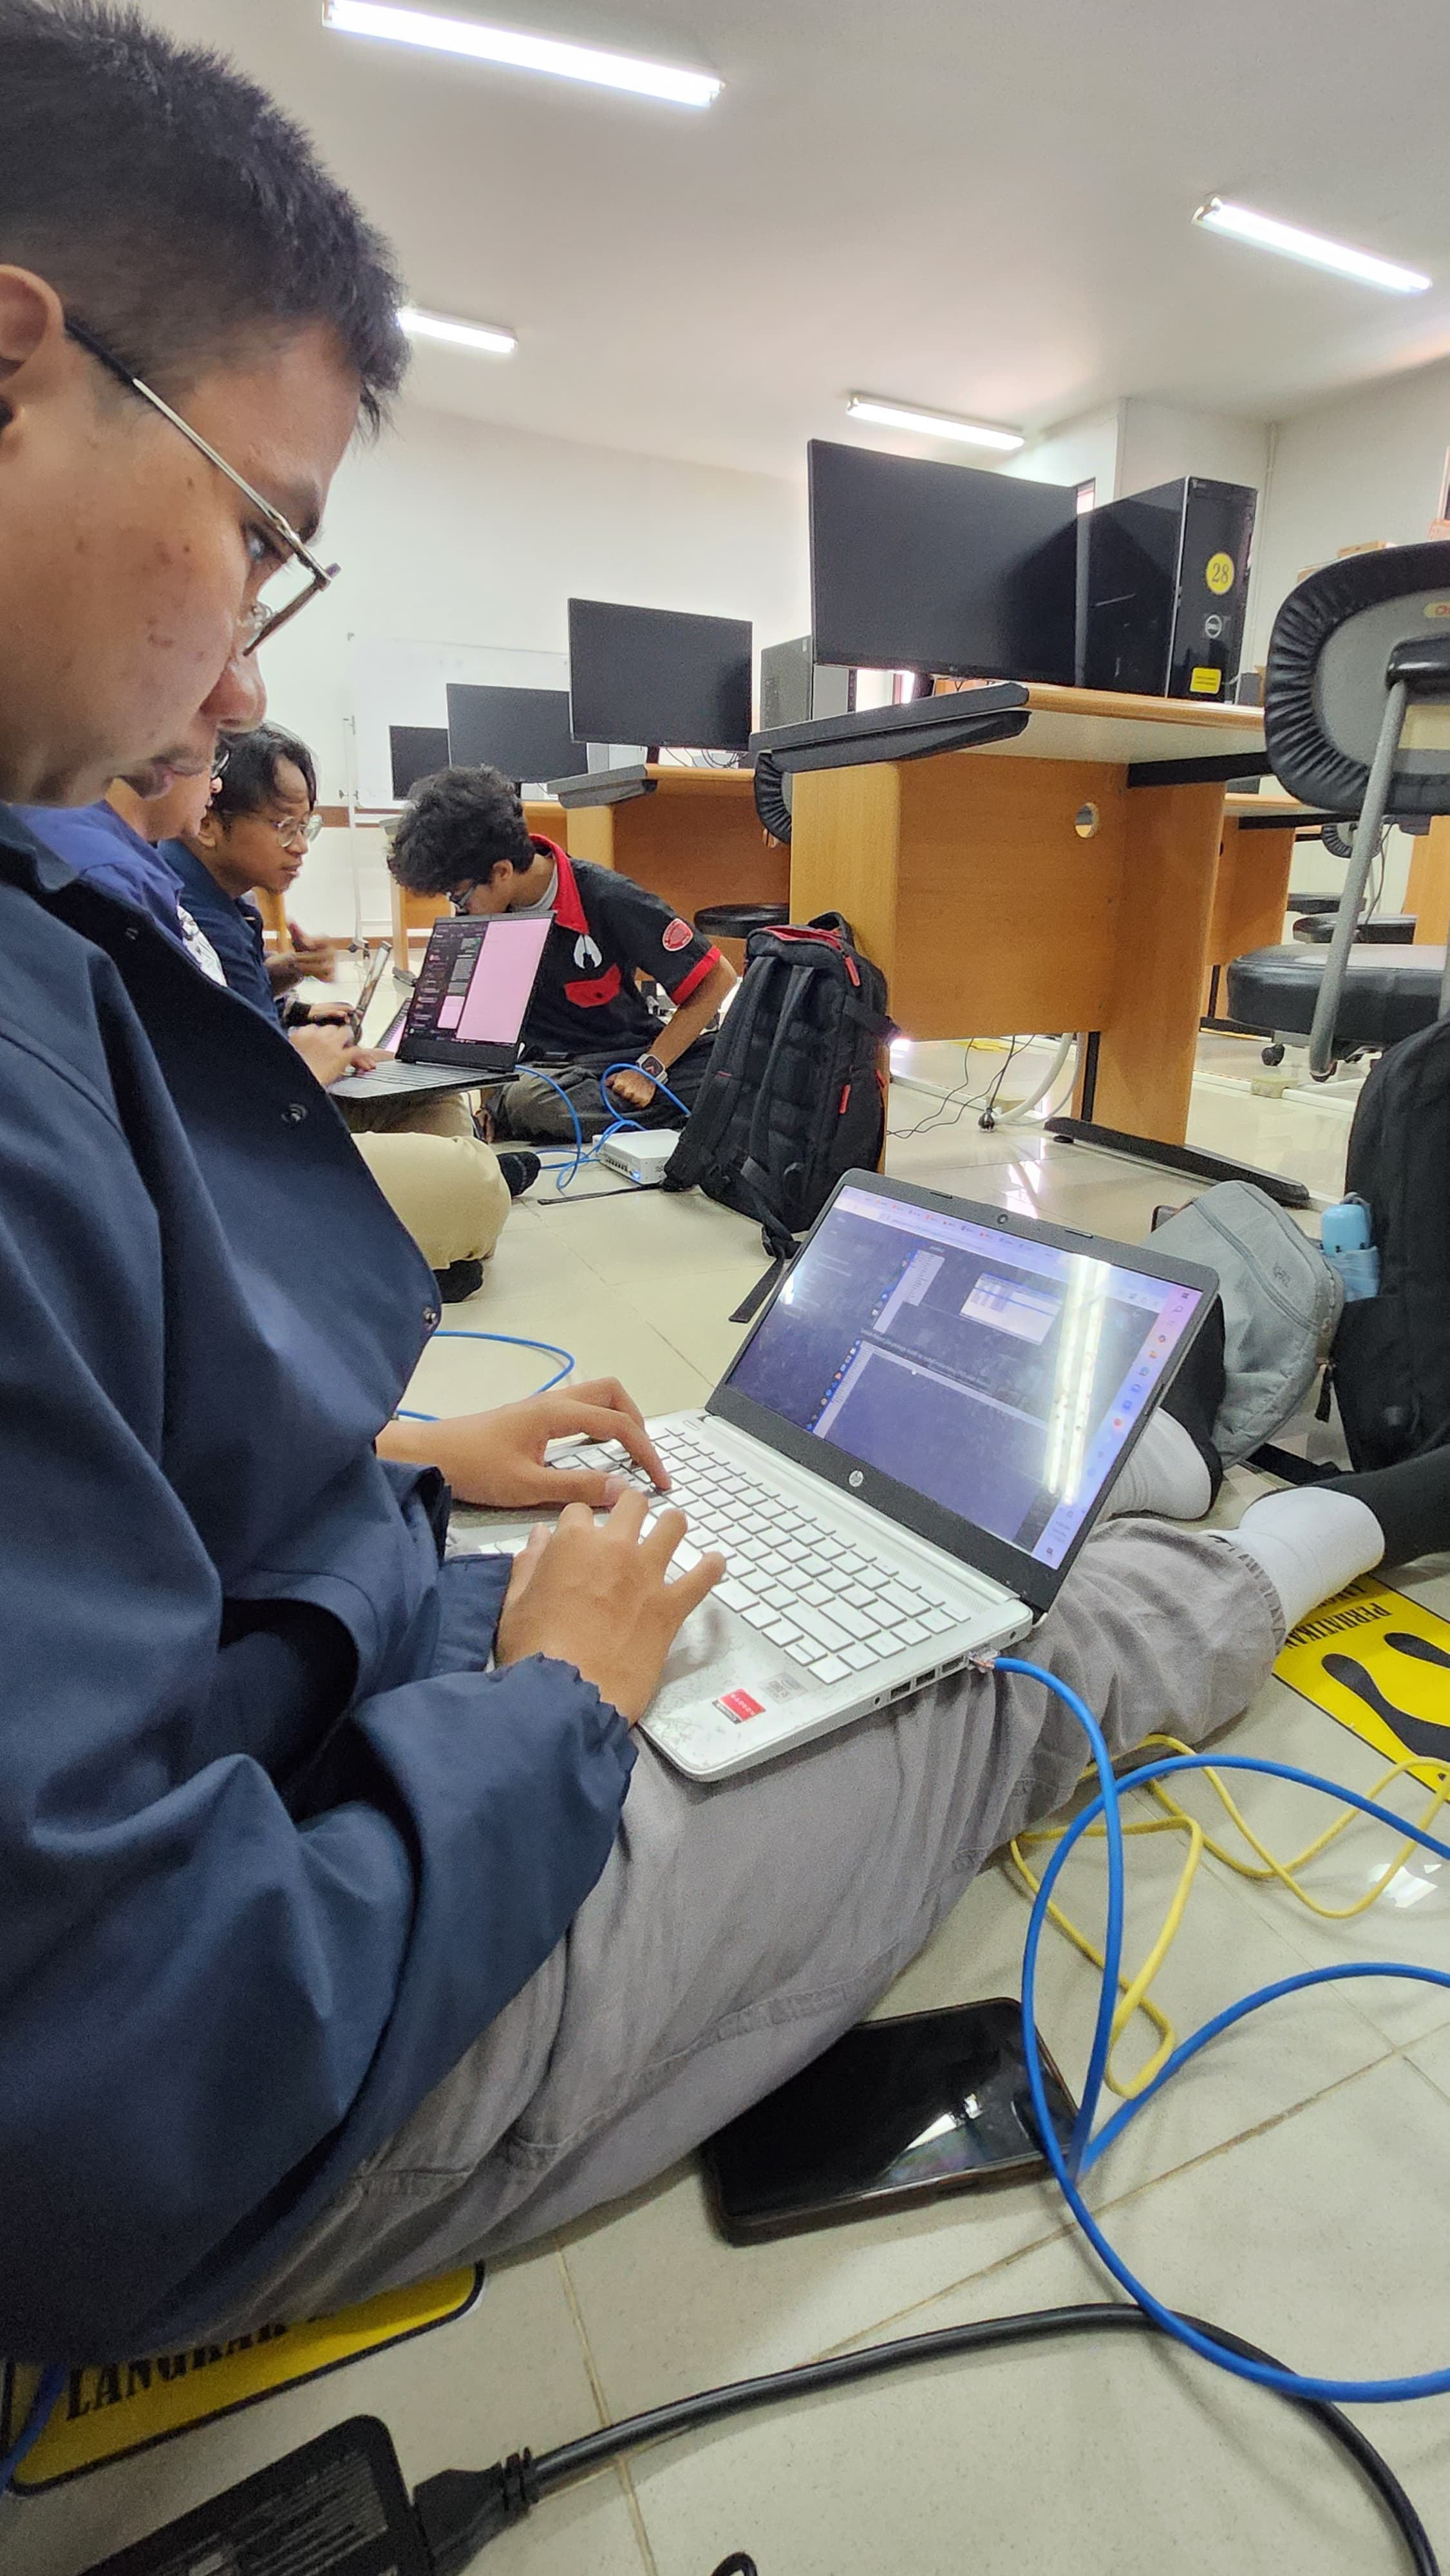
\includegraphics[width=0.5\linewidth]{P1/gambar10.jpeg}
        \caption{Dokumentasi}
        \label{fig:gambar1}
    \end{figure}

    \begin{figure}[H]
        \centering
        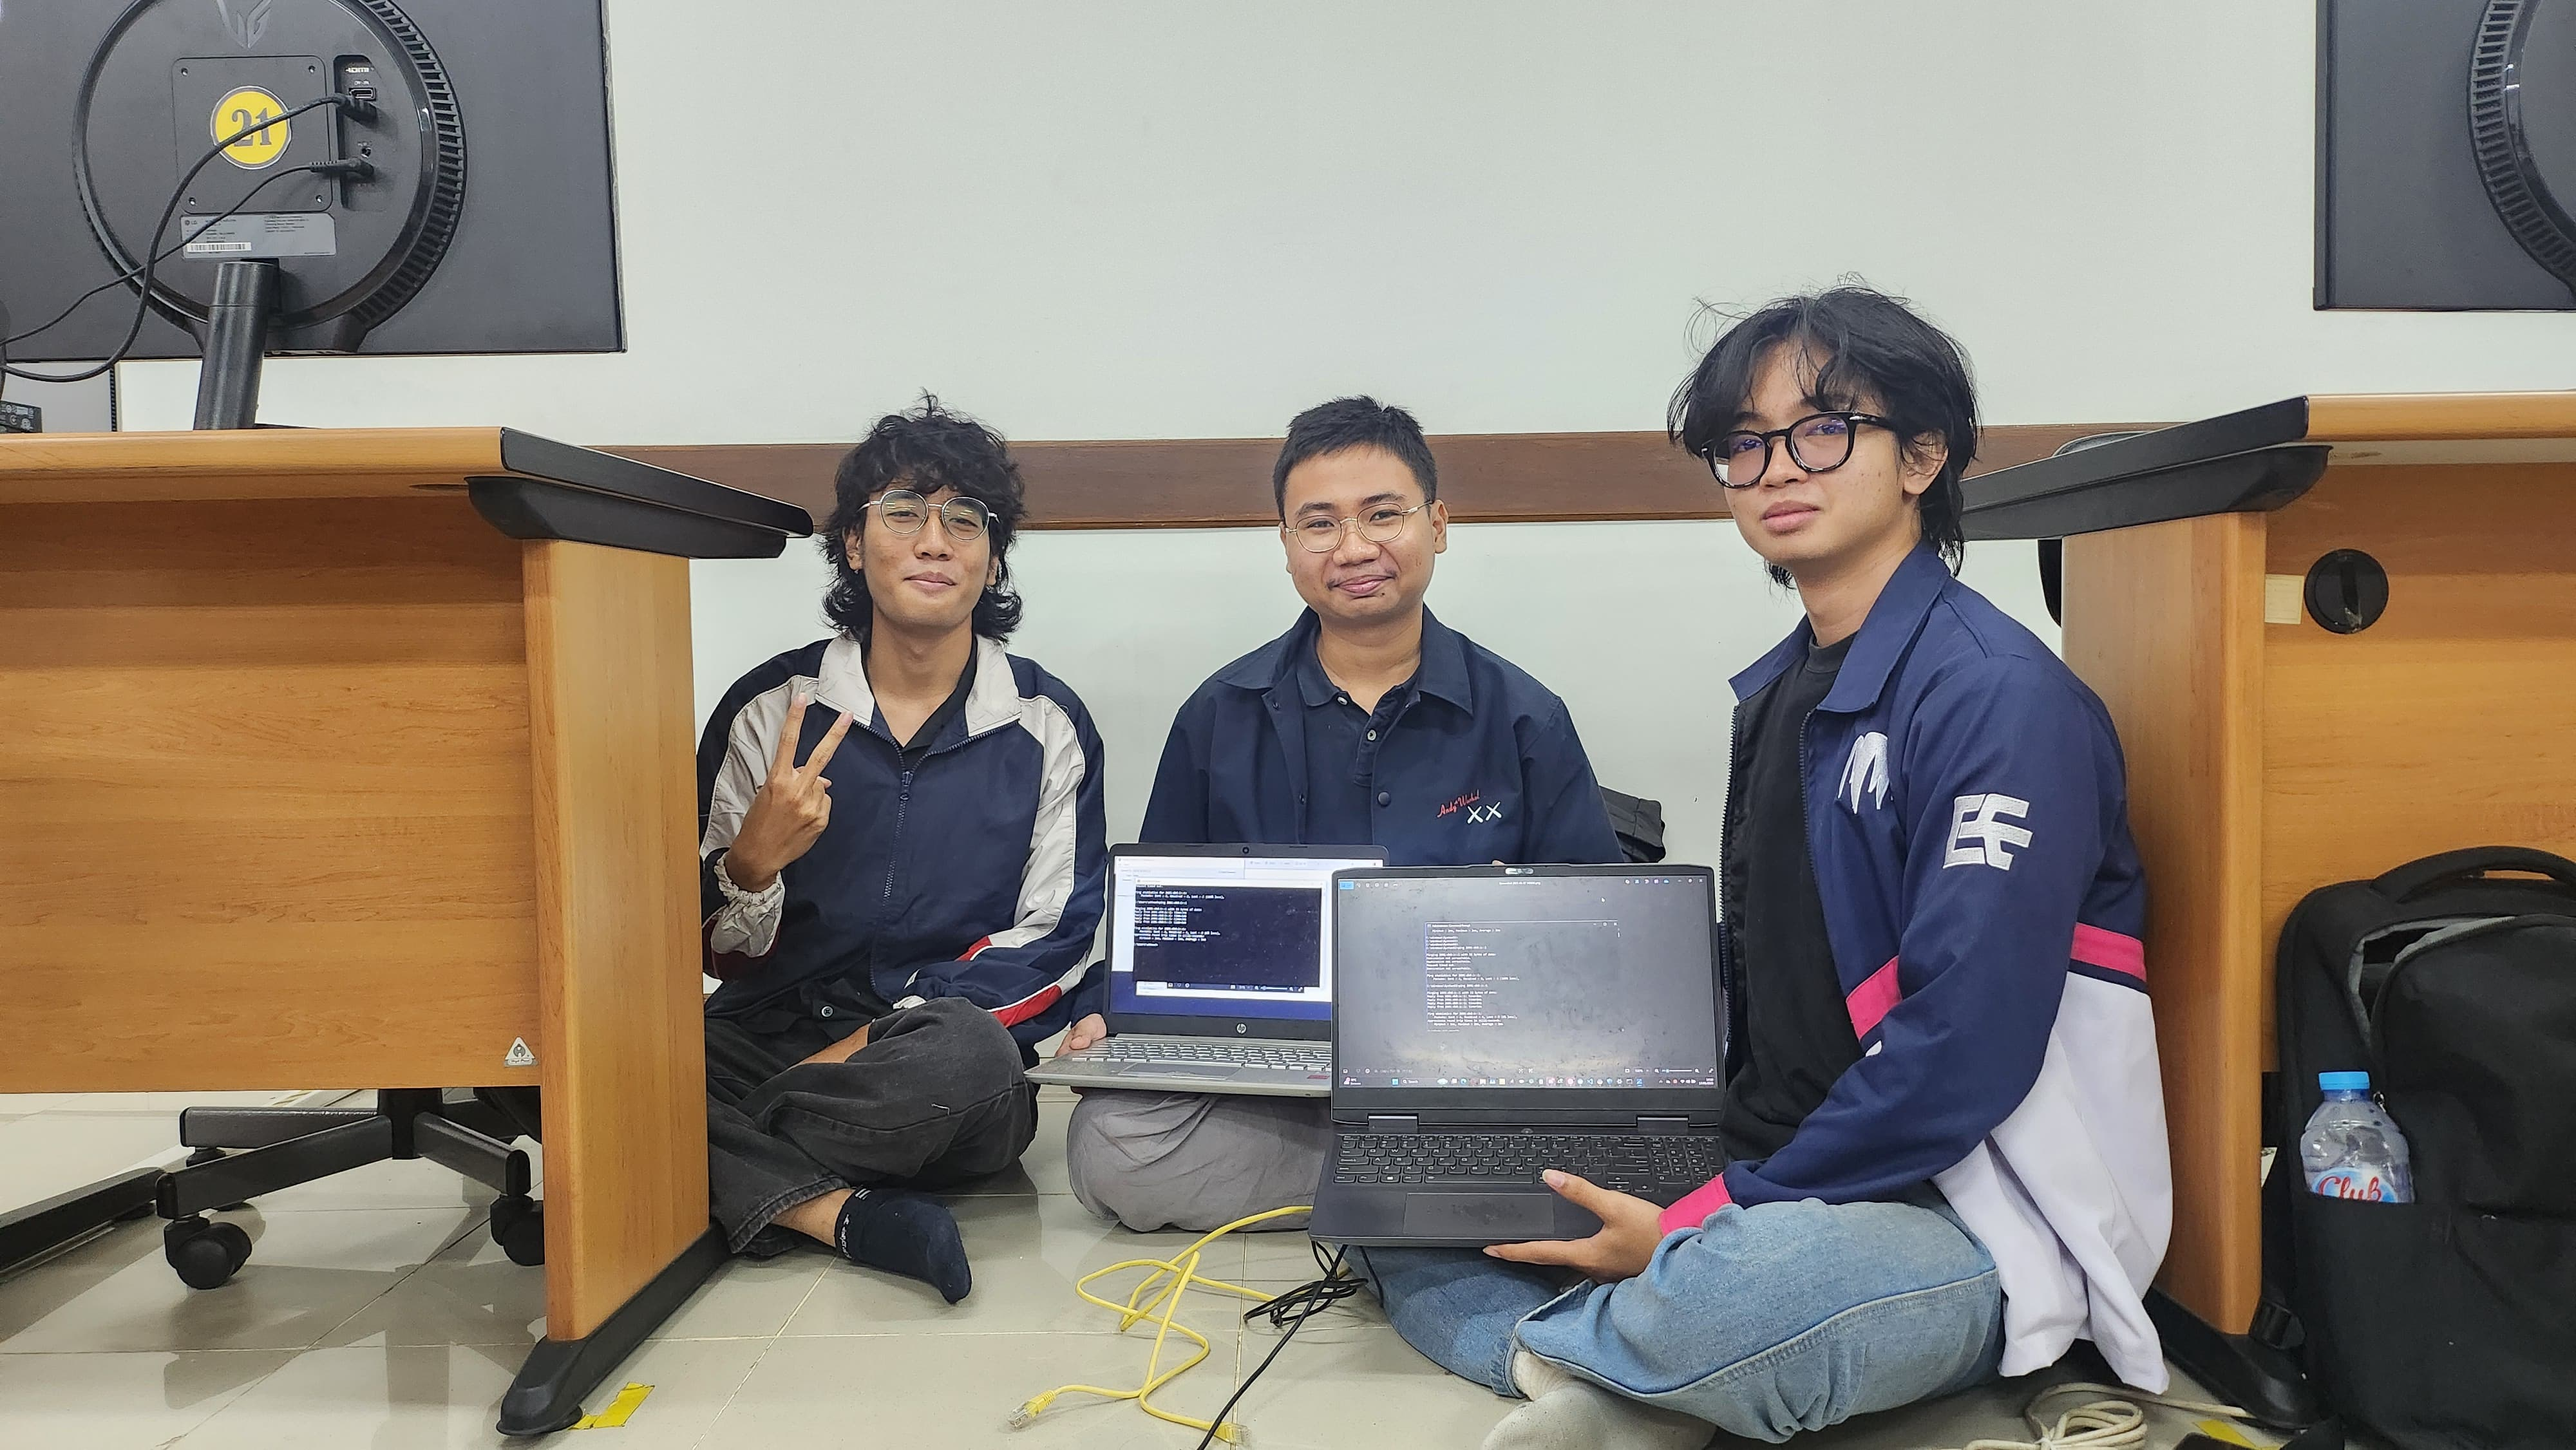
\includegraphics[width=0.5\linewidth]{P1/gambar8.jpeg}
        \caption{Dokumentasi}
        \label{fig:gambar1}
    \end{figure}

    \begin{figure}[H]
        \centering
        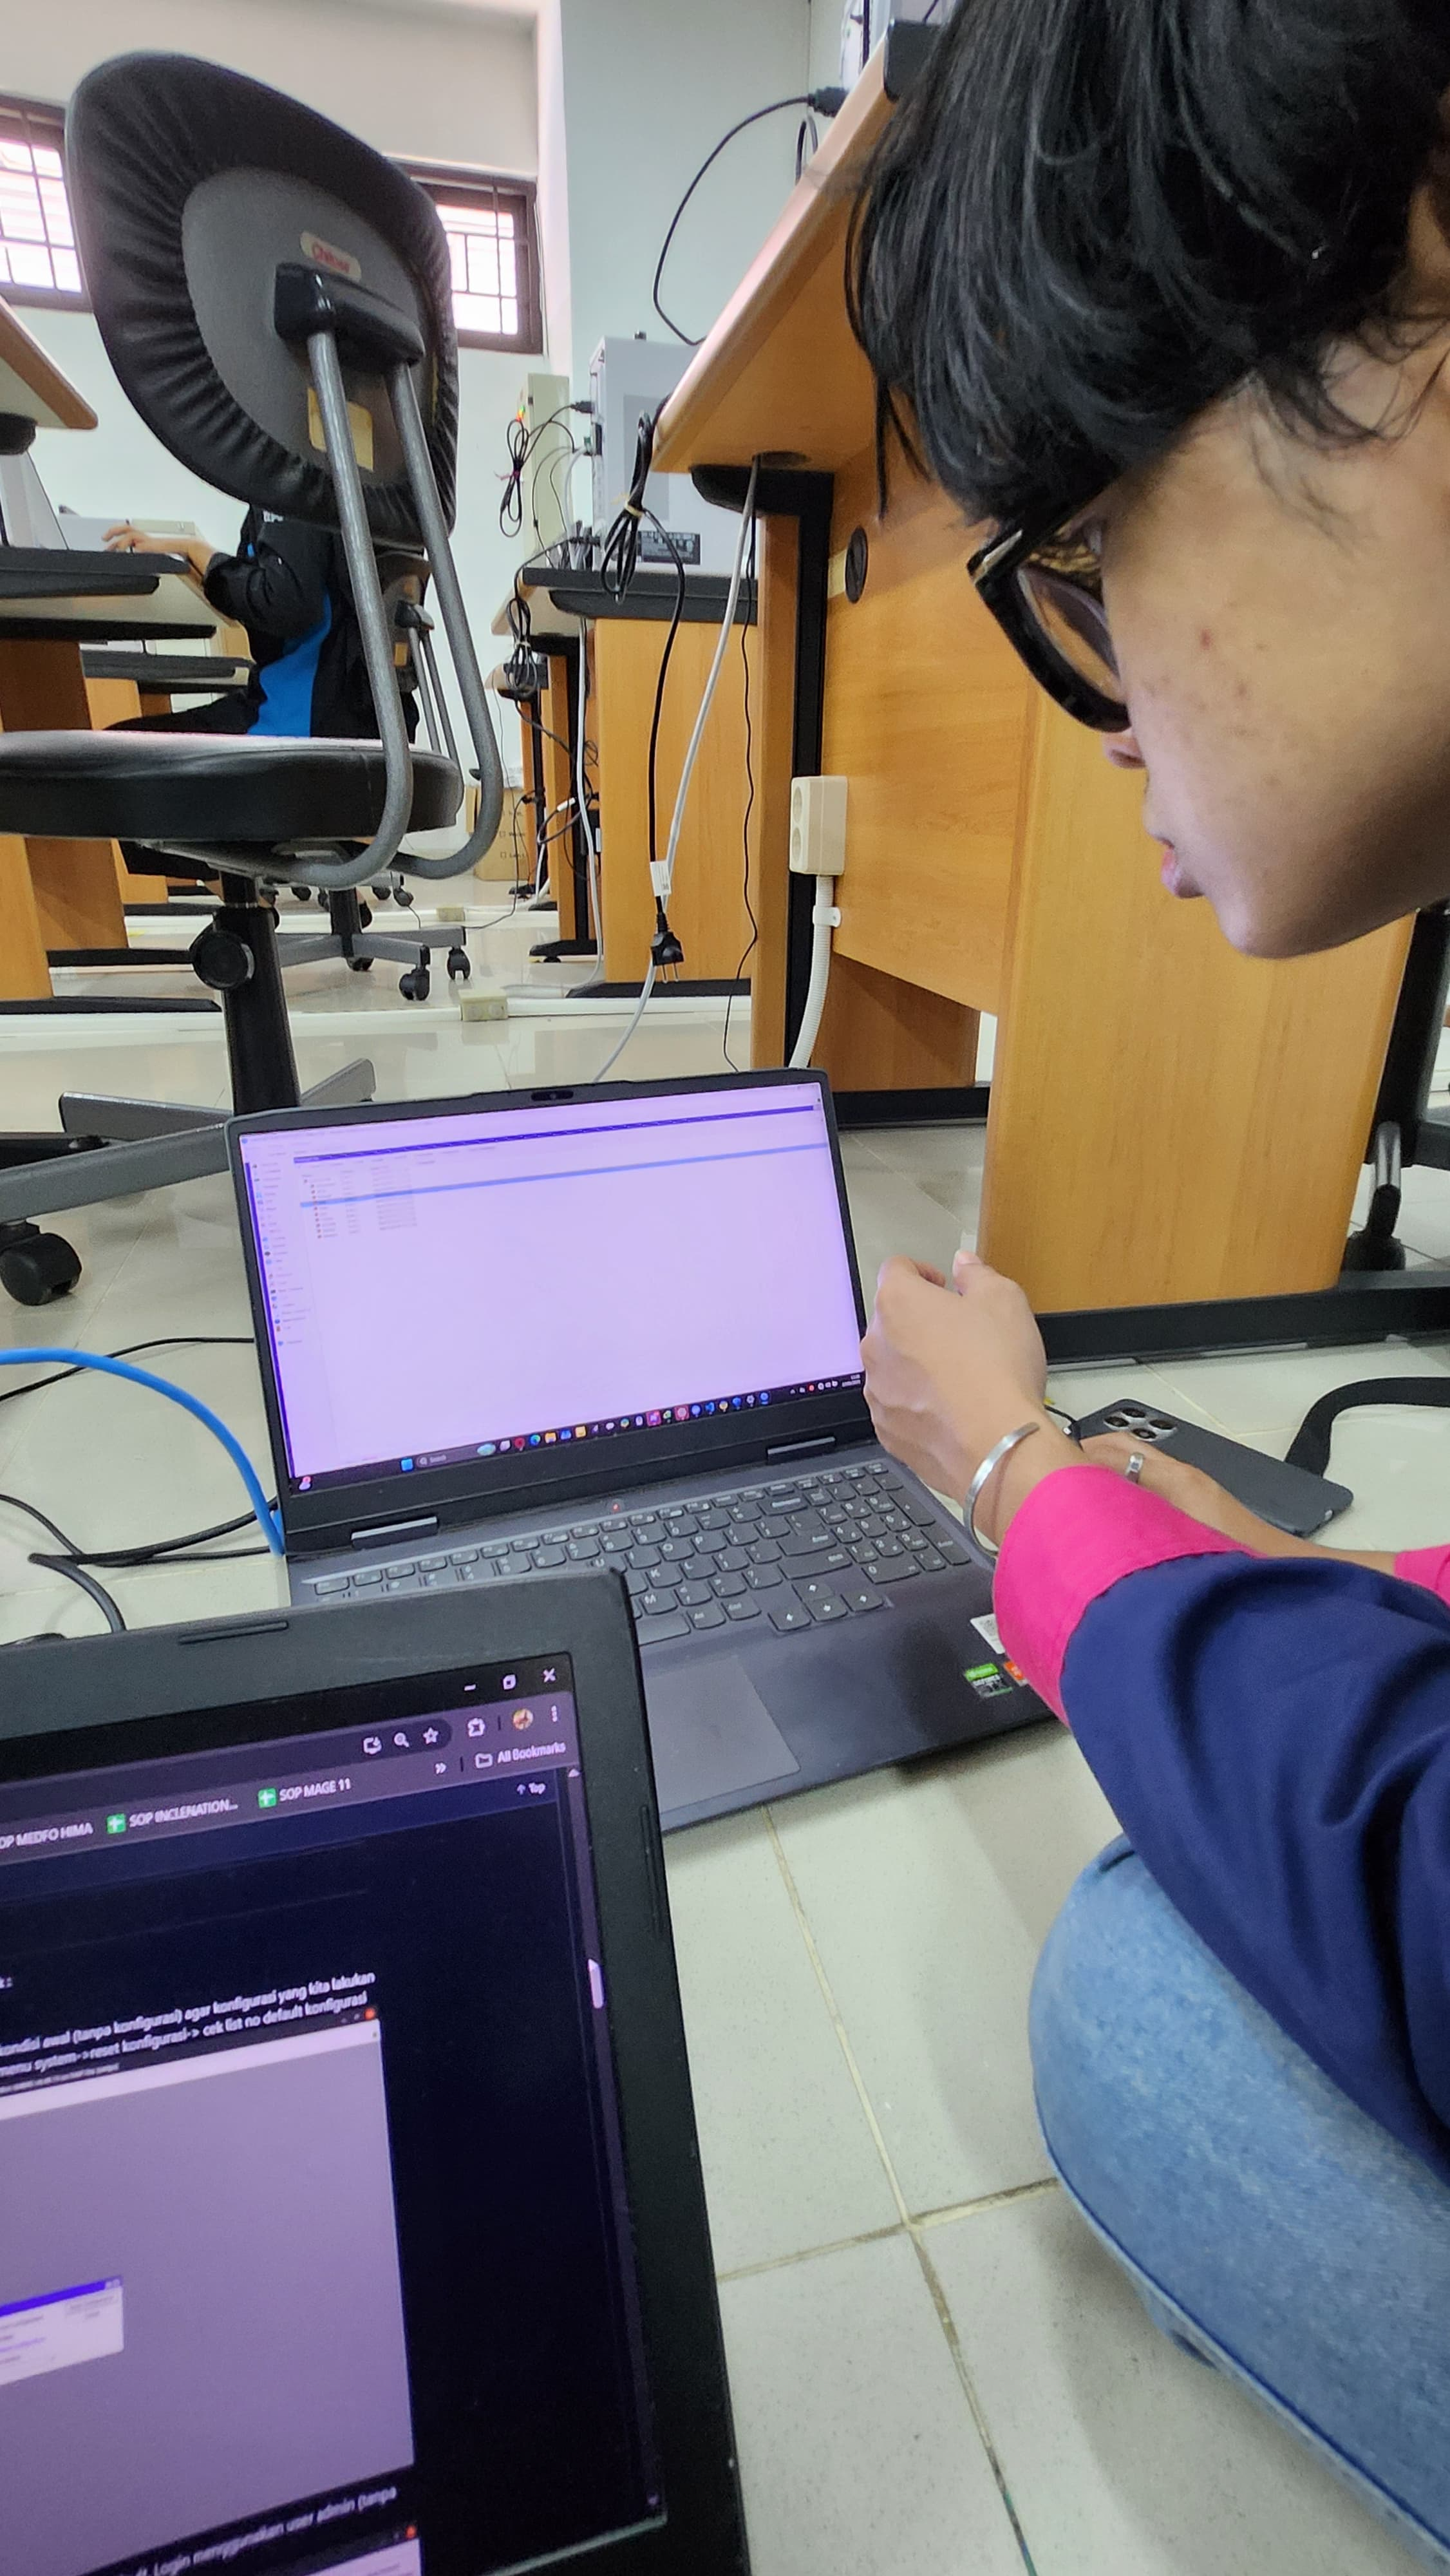
\includegraphics[width=0.5\linewidth]{P1/gambar11.jpeg}
        \caption{Dokumentasi}
        \label{fig:gambar1}
    \end{figure}

    \begin{figure}[H]
        \centering
        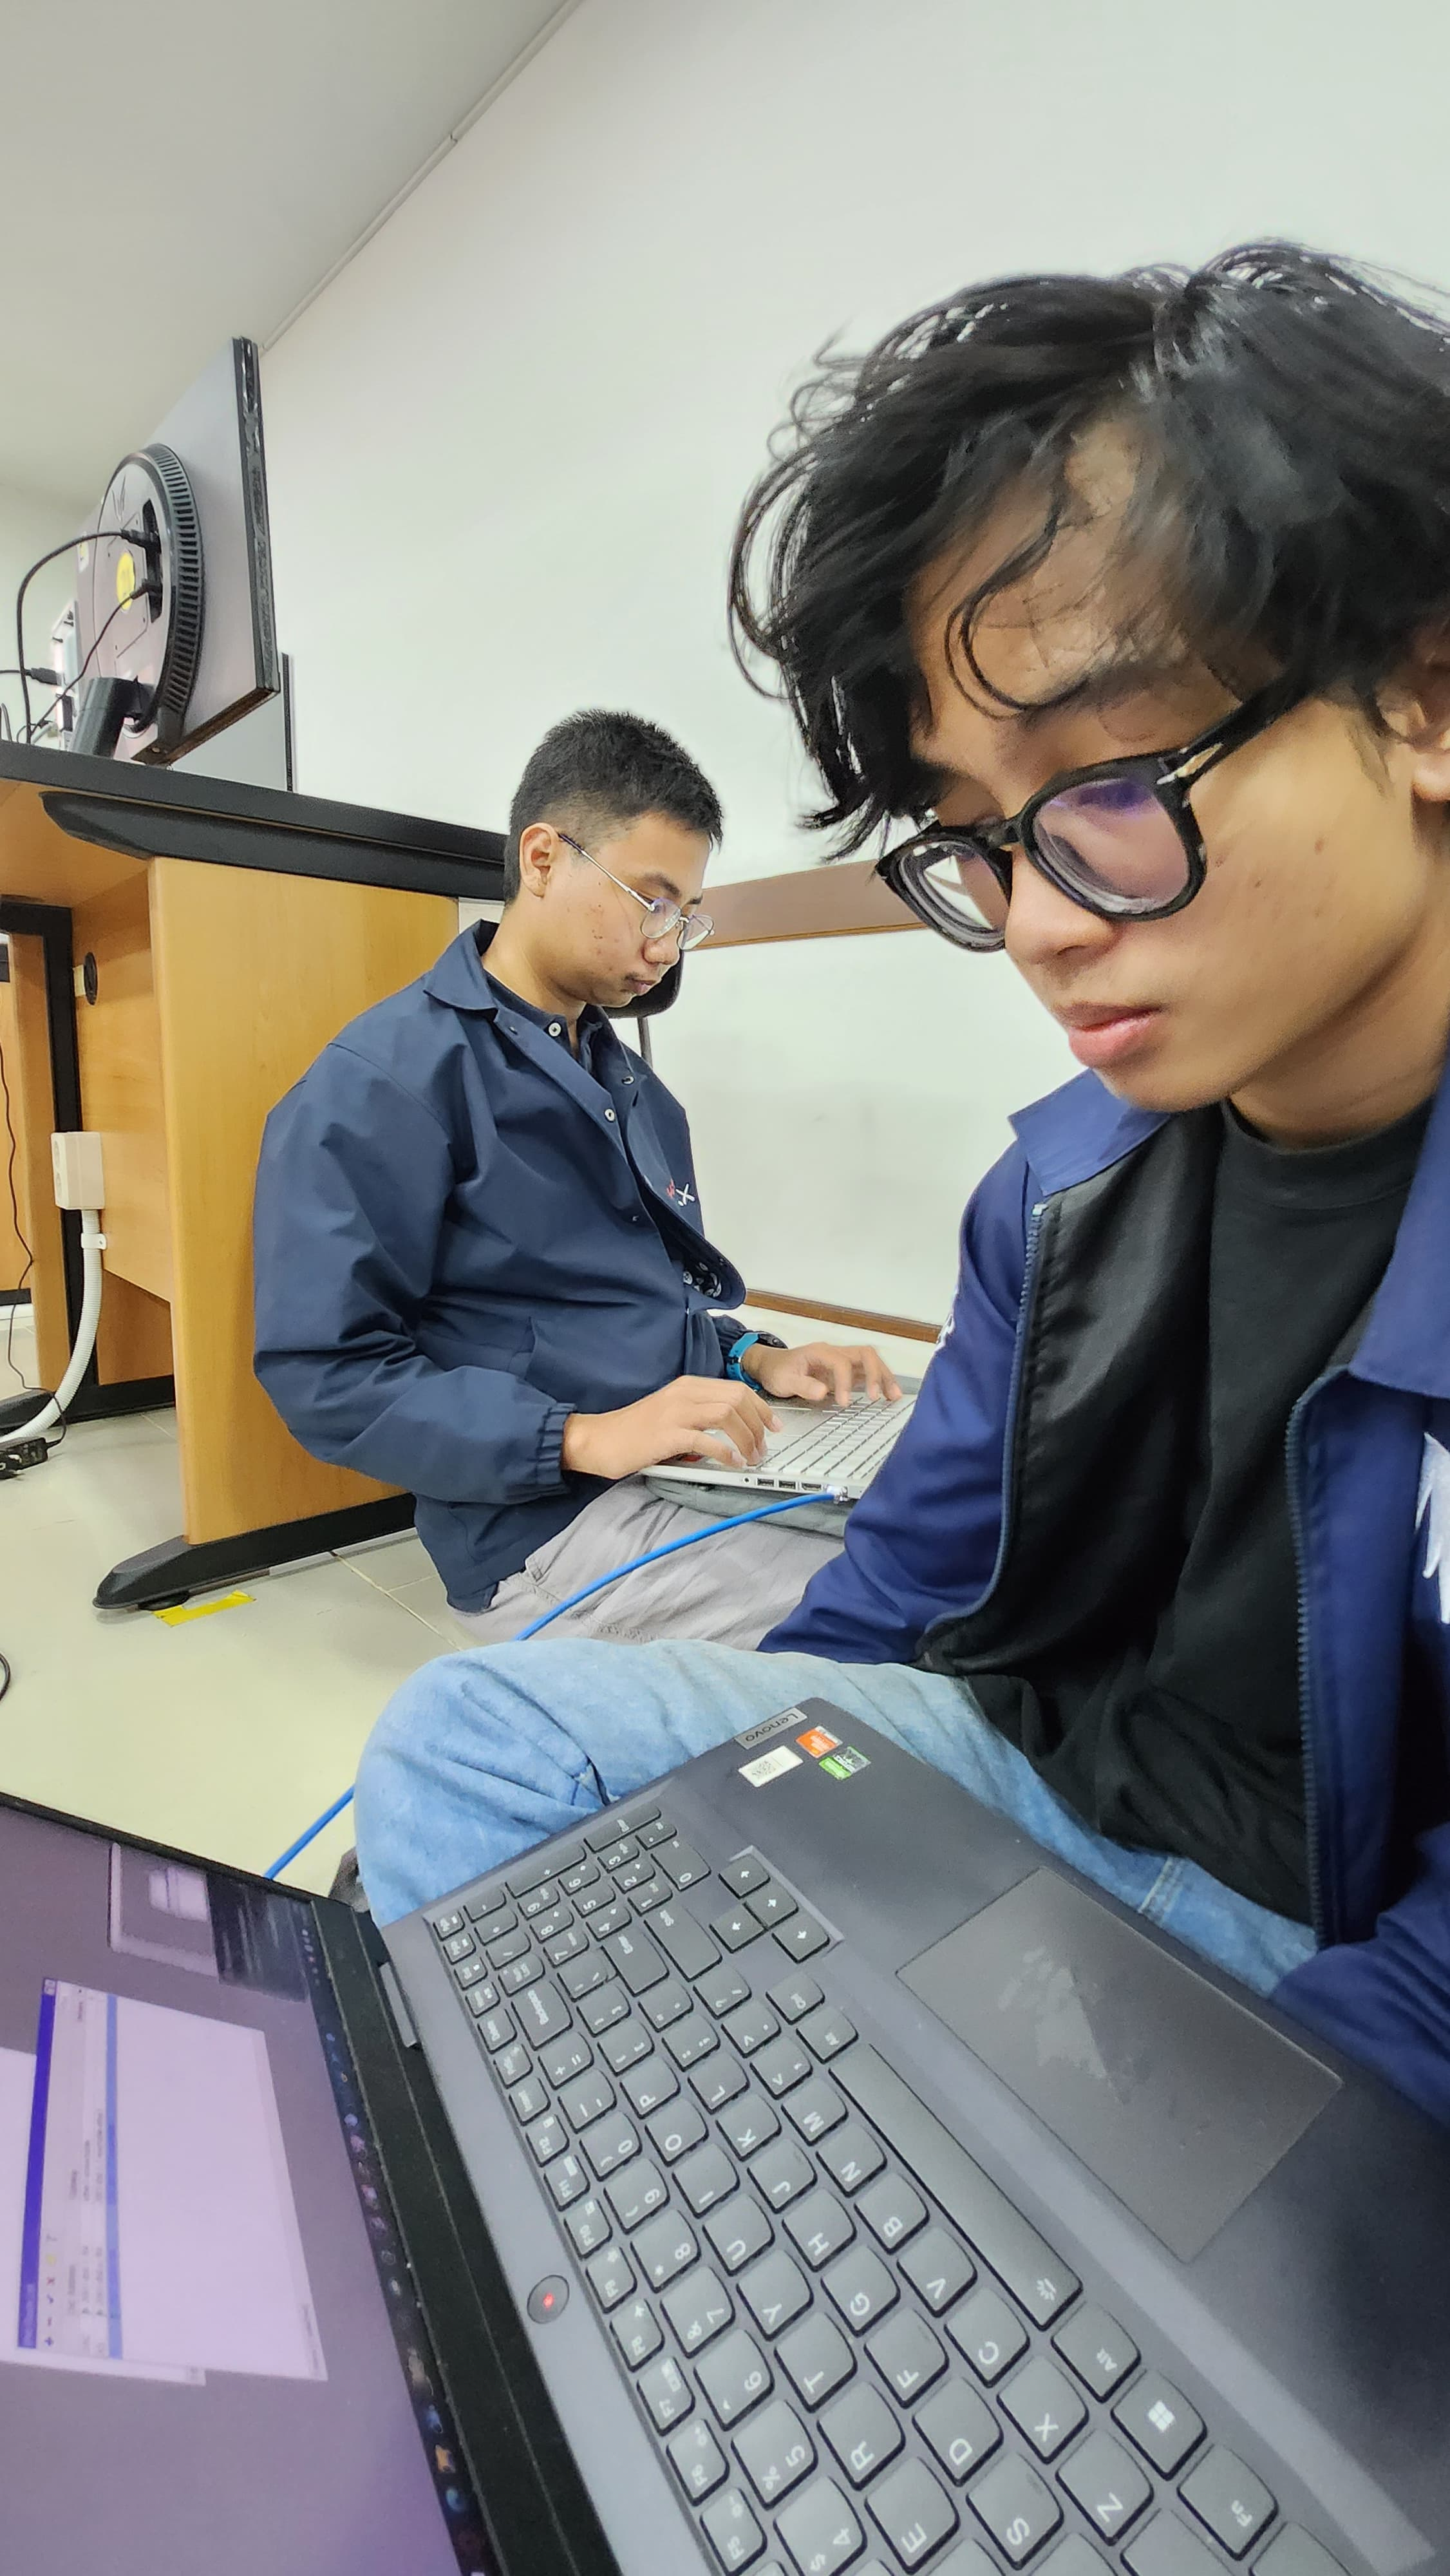
\includegraphics[width=0.5\linewidth]{P1/gambar9.jpeg}
        \caption{Dokumentasi}
        \label{fig:gambar1} 
    \end{figure}
